\documentclass[11pt]{report}

\usepackage{report}
\usepackage[utf8]{inputenc} % allow utf-8 input
\usepackage[T1]{fontenc}    % use 8-bit T1 fonts
\usepackage[colorlinks=true, linkcolor=black, citecolor=blue, urlcolor=blue]{hyperref}       % hyperlinks
\usepackage{url}            % simple URL typesetting
\usepackage{booktabs}       % professional-quality tables
\usepackage{amsfonts}       % blackboard math symbols
\usepackage{nicefrac}       % compact symbols for 1/2, etc.
\usepackage{microtype}      % microtypography
\usepackage{graphicx}
\usepackage{doi}
\usepackage{tikz}
\usepackage{amsmath}
\usepackage{amssymb}
\usepackage{chemformula}
\usepackage{listings}
\usepackage{xcolor}
\usepackage{mwe}
\usepackage{siunitx}
\usepackage{appendix}
\usepackage{setspace}
\usepackage{subcaption}

\usepackage[capitalise]{cleveref}
\creflabelformat{equation}{#2\textup{#1}#3}
\usepackage{amsthm}


\makeatletter
  \renewcommand*\tagform@[1]{\maketag@@@{Eq.~\ignorespaces #1\unskip\@@italiccorr}}
\makeatother


\definecolor{codegreen}{rgb}{0,0.6,0}
\definecolor{codegray}{rgb}{0.5,0.5,0.5}
\definecolor{codepurple}{rgb}{0.58,0,0.82}
\definecolor{backcolour}{rgb}{0.95,0.95,0.92}

\newcommand{\hly}[1]{\colorbox{yellow}{\parbox{\textwidth}{#1}}}
\newcommand\todo[1]{\textcolor{red}{#1}}


\lstdefinestyle{mystyle}{
    backgroundcolor=\color{backcolour},   
    commentstyle=\color{codegreen},
    keywordstyle=\color{magenta},
    numberstyle=\tiny\color{codegray},
    stringstyle=\color{codepurple},
    basicstyle=\ttfamily\footnotesize,
    breakatwhitespace=false,         
    breaklines=true,                 
    captionpos=b,                    
    keepspaces=true,                 
    numbers=left,                    
    numbersep=5pt,                  
    showspaces=false,                
    showstringspaces=false,
    showtabs=false,                  
    tabsize=2
}

\lstset{style=mystyle}

%% ========================
%% REMOVE BEFORE SUBMISSION
 \usepackage[angle=0, fontsize=0.03\paperwidth, vpos=0.027\paperheight, color=red]{draftwatermark}
%% ========================

%\setcitestyle{aysep={,}}
\renewcommand{\headeright}{M.Sc. Thesis}
\renewcommand{\shorttitle}{Simulating RFKO Slow Extraction}

\setlength{\parindent}{20pt}
\onehalfspacing
\begin{document}
%%%%%%%%%%%%%%%%%%%%%%%%%%%%%%%%%%%%%%%%%
% University Assignment Title Page 
% LaTeX Template
% Version 1.0 (27/12/12)
%
% This template has been downloaded from:
% http://www.LaTeXTemplates.com
%
% Original author:
% WikiBooks (http://en.wikibooks.org/wiki/LaTeX/Title_Creation)
%
% License:
% CC BY-NC-SA 3.0 (http://creativecommons.org/licenses/by-nc-sa/3.0/)
% 
% Instructions for using this template:
% This title page is capable of being compiled as is. This is not useful for 
% including it in another document. To do this, you have two options: 
%
% 1) Copy/paste everything between \begin{document} and \end{document} 
% starting at \begin{titlepage} and paste this into another LaTeX file where you 
% want your title page.
% OR
% 2) Remove everything outside the \begin{titlepage} and \end{titlepage} and 
% move this file to the same directory as the LaTeX file you wish to add it to. 
% Then add \input{./title_page_1.tex} to your LaTeX file where you want your
% title page.
%
%%%%%%%%%%%%%%%%%%%%%%%%%%%%%%%%%%%%%%%%%
%\title{Title page with logo}
%----------------------------------------------------------------------------------------
%	PACKAGES AND OTHER DOCUMENT CONFIGURATIONS
%----------------------------------------------------------------------------------------
\begin{titlepage}

\newcommand{\HRule}{\rule{\linewidth}{0.5mm}} % Defines a new command for the horizontal lines, change thickness here
\center % Center everything on the page
 
%----------------------------------------------------------------------------------------
%	HEADING SECTIONS
%----------------------------------------------------------------------------------------

\textsc{\LARGE Royal Holloway University of London}\\[1.5cm] % Name of your university/college
\textsc{\Large M.Sc Thesis}\\[0.5cm] % Major heading such as course name
\textsc{\large Student ID: 100920158}\\[0.5cm] % Minor heading such as course title

%----------------------------------------------------------------------------------------
%	TITLE SECTION
%----------------------------------------------------------------------------------------

\HRule \\[0.4cm]
\begin{spacing}{2}
{ \huge \bfseries Comparative Analysis of Simulations and Experimental Outcomes: Slow Extraction Driven by RF Transverse Excitation at the CERN Proton Synchrotron}\\[0.4cm] % Title of your document
\end{spacing}
\HRule \\[0.4cm]

 
%----------------------------------------------------------------------------------------
%	AUTHOR SECTION
%----------------------------------------------------------------------------------------

\begin{minipage}{0.4\textwidth}
\begin{flushleft} \large
\emph{Author:}\\
Thomas \textsc{Bass} % Your name
\end{flushleft}
\end{minipage}
~
\begin{minipage}{0.4\textwidth}
\begin{flushright} \large
\emph{Supervisor:} \\
Professor Stephen \textsc{Gibson} % Supervisor's Name
\end{flushright}
\end{minipage}\\[2cm]

% If you don't want a supervisor, uncomment the two lines below and remove the section above
%\Large \emph{Author:}\\
%John \textsc{Smith}\\[3cm] % Your name

%----------------------------------------------------------------------------------------
%	DATE SECTION
%----------------------------------------------------------------------------------------

{\large \today}\\[2cm] % Date, change the \today to a set date if you want to be precise

%----------------------------------------------------------------------------------------
%	LOGO SECTION
%----------------------------------------------------------------------------------------


\includegraphics[width=0.25\linewidth]{Royal_Holloway_coat_of_arms.png}\\[1cm] % Include a department/university logo - this will require the graphicx package
 
%----------------------------------------------------------------------------------------

\vfill % Fill the rest of the page with whitespace

\end{titlepage}



\newpage
\tableofcontents
\thispagestyle{empty}

\newpage
\thispagestyle{empty}
\begin{abstract}
  \setlength{\parindent}{20pt}
Resonant slow extraction is a beam extraction method which provides a continuous spill over a longer duration than can be achieved with fast single-turn or non-resonant multi-turn extraction. By using transverse excitation to drive the circulating particles onto the resonance, long-duration spills can be produced, and delivered to facilities such as fixed-target experiments, or hadron therapy gantries.

\par In order to accurately and efficiently simulate the extraction process over a wide range of timescales, new modelling tools and computing platforms must be explored. By utilising optimised computational hardware---such as General Purpose Graphics Processing Units (GPGPUs), and next-generation simulation software (such as \verb|Xsuite|), computation times for simulations can be reduced by several orders of magnitude.

\par This thesis presents recent developments of resonant slow extraction modelling and benchmarking with a comparison to measurements made at CERN’s Proton Synchrotron (PS), with a particular focus on understanding the dynamics of transverse RF excitation and effect on spill quality.

\end{abstract}
\vspace*{\fill}
\keywords{Beam Physics, Slow Extraction, Radio-Frequency Knock-Out, Simulation, Xsuite}
\vspace*{\fill}
\newpage
%\setcounter{page}{1}
\chapter{Introduction}


The CERN Proton Synchrotron (PS), alongside providing intermediary acceleration for hadron and ion beams for the Super Proton Synchrotron (SPS) and eventually the Large Hadron Collider (LHC), provides beams for the many fixed target experiments located at the East Area (EA) experimental facility. This facility, as illustrated in~\autoref{fig:eadiagram}, consists of the proton (IRRAD) and mixed-field (CHARM) irradiation facilities, via a dedicated \qty{24}{GeV/c} beamline, in addition to a multi-target beamline providing three secondary beams.

Ongoing experiments in these facilities such as the CHARM High-energy Ions for Micro Electronics Reliability Assurance (CHIMERA)~\cite{Fraser:feasibility} use high-Z ions (Pb) to simulate the harsh radiation environment of cosmic rays which satellites experience. Using low-intensity (\qty{<e6}{ions/spill}), high-energy (\qty{>100}{\MeV / u}) beams, customers such as the European Space Agency can assess the reliability of new materials in these environments.~\autoref{fig:chain} illustrates the two injection chains of the PS, either with Lead ions sourced from the Linear Accelerator 3 (Linac3) and Low Energy Ion Ring (LEIR) chain, or protons from the Linac4 and the Proton Synchrotron Booster (PSB).

\begin{figure}
  \tikzset{every picture/.style={line width=0.75pt}} %set default line width to 0.75pt        

  \begin{tikzpicture}[x=0.75pt,y=0.75pt,yscale=-1,xscale=1]
  %uncomment if require: \path (0,300); %set diagram left start at 0, and has height of 300
  
  %Shape: Arc [id:dp13623924019589717] 
  \draw  [draw opacity=0][line width=3]  (23.16,157.13) .. controls (40.51,146.27) and (61.02,140) .. (83,140) .. controls (145.41,140) and (196,190.59) .. (196,253) .. controls (196,257.08) and (195.78,261.12) .. (195.36,265.09) -- (83,253) -- cycle ; \draw  [line width=3]  (23.16,157.13) .. controls (40.51,146.27) and (61.02,140) .. (83,140) .. controls (145.41,140) and (196,190.59) .. (196,253) .. controls (196,257.08) and (195.78,261.12) .. (195.36,265.09) ;  
  %Straight Lines [id:da9881615579049192] 
  \draw [line width=3]    (80,140) -- (540,140) ;
  %Curve Lines [id:da41561885076946403] 
  \draw [line width=3]    (160,140) .. controls (220.2,139.6) and (190.2,178.6) .. (260,180) ;
  %Straight Lines [id:da9738553160260242] 
  \draw [line width=3]    (260,170) -- (260,190) ;
  %Curve Lines [id:da062105937338959416] 
  \draw [line width=3]    (160,140) .. controls (220.2,139.6) and (190.2,98.6) .. (260,100) ;
  %Curve Lines [id:da9621165186674936] 
  \draw [line width=3]    (260,100) .. controls (320.2,99.6) and (320.2,68.6) .. (390,70) ;
  %Curve Lines [id:da22957973507324092] 
  \draw [line width=3]    (260,100) .. controls (320.2,99.6) and (470.2,98.6) .. (540,100) ;
  %Curve Lines [id:da814674780127862] 
  \draw [line width=3]    (390,70) .. controls (450.2,69.6) and (418.8,38.6) .. (540,40) ;
  %Curve Lines [id:da1370169663287728] 
  \draw [line width=3]    (390,70) .. controls (450.2,69.6) and (470.2,68.6) .. (540,70) ;
  %Shape: Parallelogram [id:dp6647261304834908] 
  \draw  [fill={rgb, 255:red, 80; green, 227; blue, 194 }  ,fill opacity=1 ] (477.7,30) -- (540,30) -- (532.3,50) -- (470,50) -- cycle ;
  %Shape: Parallelogram [id:dp21515901263901416] 
  \draw  [fill={rgb, 255:red, 80; green, 227; blue, 194 }  ,fill opacity=1 ] (367.7,129) -- (430,129) -- (422.3,149) -- (360,149) -- cycle ;
  %Shape: Parallelogram [id:dp5134940082894275] 
  \draw  [fill={rgb, 255:red, 80; green, 227; blue, 194 }  ,fill opacity=1 ] (457.7,129) -- (520,129) -- (512.3,149) -- (450,149) -- cycle ;
  \draw  [fill={rgb, 255:red, 0; green, 0; blue, 0 }  ,fill opacity=1 ] (206,240) -- (196,260) -- (186,240) -- (196,250) -- cycle ;
  \draw  [fill={rgb, 255:red, 0; green, 0; blue, 0 }  ,fill opacity=1 ] (139,130) -- (159,140) -- (139,150) -- (149,140) -- cycle ;
  
  % Text Node
  \draw (151,120) node [anchor=north west][inner sep=0.75pt]   [align=left] {F61};
  % Text Node
  \draw (271,171) node [anchor=north west][inner sep=0.75pt]   [align=left] {F6D East Dump};
  % Text Node
  \draw (551,132) node [anchor=north west][inner sep=0.75pt]   [align=left] {T8 24 GeV/c};
  % Text Node
  \draw (241,82) node [anchor=north west][inner sep=0.75pt]   [align=left] {F62};
  % Text Node
  \draw (371,52) node [anchor=north west][inner sep=0.75pt]   [align=left] {F63};
  % Text Node
  \draw (551,32) node [anchor=north west][inner sep=0.75pt]   [align=left] {T11 3.5 GeV/c};
  % Text Node
  \draw (551,62) node [anchor=north west][inner sep=0.75pt]   [align=left] {T10 7 GeV/c};
  % Text Node
  \draw (551,92) node [anchor=north west][inner sep=0.75pt]   [align=left] {T9 15 GeV/c};
  % Text Node
  \draw (478.7,32) node [anchor=north west][inner sep=0.75pt]   [align=left] {CLOUD};
  % Text Node
  \draw (371.7,131) node [anchor=north west][inner sep=0.75pt]   [align=left] {IRRAD};
  % Text Node
  \draw (456.7,131) node [anchor=north west][inner sep=0.75pt]   [align=left] {CHARM};
  % Text Node
  \draw (114,246) node [anchor=north west][inner sep=0.75pt]   [align=left] {CERN PS};
  
  
  \end{tikzpicture}
  
\caption{Layout diagram of the CERN East Area (EA) beamlines, their proton momenta, and experiments.}\label{fig:eadiagram}
\end{figure}

\begin{figure}
  \centering
    \tikzset{every picture/.style={line width=0.75pt}} %set default line width to 0.75pt        
    \begin{tikzpicture}[x=0.75pt,y=0.75pt,yscale=-1,xscale=1]
    %uncomment if require: \path (0,715); %set diagram left start at 0, and has height of 715
    %Curve Lines [id:da12691543918942427] 
    \draw [line width=3]    (402.5,510) .. controls (308.4,510.6) and (214.4,353.6) .. (212.4,293.6) ;
    %Curve Lines [id:da8510608919978877] 
    \draw [color={rgb, 255:red, 255; green, 255; blue, 255 }  ,draw opacity=1 ][line width=6]    (230,480) .. controls (274.2,480.4) and (281.4,441.8) .. (301.2,406.2) ;
    %Curve Lines [id:da7502083546431804] 
    \draw [line width=3]    (292.5,365) .. controls (329.8,368.6) and (340.8,338.6) .. (402.5,335) ;
    %Curve Lines [id:da14243393865149923] 
    \draw [color={rgb, 255:red, 255; green, 255; blue, 255 }  ,draw opacity=1 ][line width=6]    (301.2,406.2) .. controls (310.2,387.2) and (334,364.5) .. (330,327.5) ;
    %Curve Lines [id:da9690549021376971] 
    \draw [line width=3]    (543.4,398) .. controls (503.4,397) and (515.2,402.2) .. (455.2,351.2) ;
    %Curve Lines [id:da18378599113206628] 
    \draw [color={rgb, 255:red, 255; green, 255; blue, 255 }  ,draw opacity=1 ][line width=6]    (299,536) .. controls (353.8,538.6) and (318.8,481.6) .. (315,422.5) ;
    %Curve Lines [id:da36505385427145587] 
    \draw [line width=3]    (184,195.8) .. controls (238,240.8) and (289,280.8) .. (423.4,282.8) ;
    %Curve Lines [id:da4662172894678054] 
    \draw [color={rgb, 255:red, 255; green, 255; blue, 255 }  ,draw opacity=1 ][line width=6]    (212.4,293.6) .. controls (211.4,225.6) and (303.4,216.6) .. (297,156.4) ;
    %Straight Lines [id:da6403083893101353] 
    \draw [line width=3]    (221,536.6) -- (285,536.2) ;
    \draw  [fill={rgb, 255:red, 0; green, 0; blue, 0 }  ,fill opacity=1 ] (238,526.6) -- (258,536.6) -- (238,546.6) -- (248,536.6) -- cycle ;
    %Curve Lines [id:da1754170813900049] 
    \draw [line width=3]    (230,480) .. controls (274.2,480.4) and (281.4,441.8) .. (301.2,406.2) ;
    %Shape: Parallelogram [id:dp9764670224277929] 
    \draw  [fill={rgb, 255:red, 248; green, 200; blue, 220 }  ,fill opacity=1 ] (165.24,468.7) -- (240,468.7) -- (230.76,489.3) -- (156,489.3) -- cycle ;
    %Shape: Circle [id:dp8387090420566679] 
    \draw  [line width=3]  (315,422.5) .. controls (315,374.18) and (354.18,335) .. (402.5,335) .. controls (450.82,335) and (490,374.18) .. (490,422.5) .. controls (490,470.82) and (450.82,510) .. (402.5,510) .. controls (354.18,510) and (315,470.82) .. (315,422.5) -- cycle ;

    %Shape: Parallelogram [id:dp16681512555108147] 
    \draw  [fill={rgb, 255:red, 200; green, 209; blue, 248 }  ,fill opacity=1 ] (154.24,525.1) -- (229,525.1) -- (219.76,545.7) -- (145,545.7) -- cycle ;
    %Rounded Rect [id:dp7810492177412798] 
    \draw  [line width=3]  (264,553.2) .. controls (264,543.81) and (271.61,536.2) .. (281,536.2) -- (340,536.2) .. controls (349.39,536.2) and (357,543.81) .. (357,553.2) -- (357,573.2) .. controls (357,582.59) and (349.39,590.2) .. (340,590.2) -- (281,590.2) .. controls (271.61,590.2) and (264,582.59) .. (264,573.2) -- cycle ;

    %Shape: Circle [id:dp8690695581292782] 
    \draw  [line width=3]  (255,327.5) .. controls (255,306.79) and (271.79,290) .. (292.5,290) .. controls (313.21,290) and (330,306.79) .. (330,327.5) .. controls (330,348.21) and (313.21,365) .. (292.5,365) .. controls (271.79,365) and (255,348.21) .. (255,327.5) -- cycle ;

    %Curve Lines [id:da8738392345224177] 
    \draw [line width=3]    (299,536) .. controls (353.8,538.6) and (318.8,481.6) .. (315,422.5) ;
    %Curve Lines [id:da06171309257415403] 
    \draw [line width=3]    (301.2,406.2) .. controls (310.2,387.2) and (334,364.5) .. (330,327.5) ;
    %Shape: Circle [id:dp2990909311240957] 
    \draw  [line width=3]  (297,156.4) .. controls (297,86.59) and (353.59,30) .. (423.4,30) .. controls (493.21,30) and (549.8,86.59) .. (549.8,156.4) .. controls (549.8,226.21) and (493.21,282.8) .. (423.4,282.8) .. controls (353.59,282.8) and (297,226.21) .. (297,156.4) -- cycle ;

    %Curve Lines [id:da4359851548001026] 
    \draw [line width=3]    (212.4,293.6) .. controls (211.4,225.6) and (303.4,216.6) .. (297,156.4) ;
    %Curve Lines [id:da274114148545888] 
    \draw [line width=3]    (591.4,278.2) .. controls (570.4,233.2) and (545,228.8) .. (549.8,156.4) ;
    \draw  [fill={rgb, 255:red, 0; green, 0; blue, 0 }  ,fill opacity=1 ] (255.98,465.42) -- (276.1,455.68) -- (271.82,477.62) -- (270,463.6) -- cycle ;
    \draw  [fill={rgb, 255:red, 0; green, 0; blue, 0 }  ,fill opacity=1 ] (234.46,385.29) -- (232.92,362.98) -- (251.69,375.14) -- (238,371.6) -- cycle ;
    \draw  [fill={rgb, 255:red, 0; green, 0; blue, 0 }  ,fill opacity=1 ] (298.27,275.28) -- (282.53,259.4) -- (304.68,256.33) -- (292,262.6) -- cycle ;
    \draw  [fill={rgb, 255:red, 0; green, 0; blue, 0 }  ,fill opacity=1 ] (575.52,230.9) -- (577.09,253.21) -- (558.3,241.08) -- (572,244.6) -- cycle ;
    \draw  [fill={rgb, 255:red, 0; green, 0; blue, 0 }  ,fill opacity=1 ] (319.57,521.14) -- (328.45,500.62) -- (339.54,520.03) -- (329,510.6) -- cycle ;
    \draw  [fill={rgb, 255:red, 0; green, 0; blue, 0 }  ,fill opacity=1 ] (264.87,317.47) -- (255.13,337.6) -- (244.87,317.73) -- (255,327.6) -- cycle ;
    \draw  [fill={rgb, 255:red, 0; green, 0; blue, 0 }  ,fill opacity=1 ] (499.87,415.47) -- (490.13,435.6) -- (479.87,415.73) -- (490,425.6) -- cycle ;
    \draw  [fill={rgb, 255:red, 0; green, 0; blue, 0 }  ,fill opacity=1 ] (292.5,118.22) -- (307.94,102.04) -- (311.62,124.1) -- (305,111.6) -- cycle ;
    %Shape: Parallelogram [id:dp44568506950093134] 
    \draw  [fill={rgb, 255:red, 80; green, 227; blue, 194 }  ,fill opacity=1 ] (542.7,386.6) -- (605,386.6) -- (597.3,406.6) -- (535,406.6) -- cycle ;

    %Curve Lines [id:da33904147754615943] 
    \draw [line width=3]    (576.4,91.2) .. controls (536.4,90.2) and (541.3,35) .. (423.4,30) ;
    %Shape: Parallelogram [id:dp12091233534601331] 
    \draw  [fill={rgb, 255:red, 80; green, 227; blue, 194 }  ,fill opacity=1 ] (576.05,81.1) -- (638.35,81.1) -- (630.65,101.1) -- (568.35,101.1) -- cycle ;

    %Shape: Parallelogram [id:dp5163558794702339] 
    \draw  [fill={rgb, 255:red, 245; green, 166; blue, 35 }  ,fill opacity=1 ] (565.7,272.5) -- (628,272.5) -- (620.3,292.5) -- (558,292.5) -- cycle ;

    %Shape: Parallelogram [id:dp272340165402827] 
    \draw  [fill={rgb, 255:red, 245; green, 166; blue, 35 }  ,fill opacity=1 ] (159.7,179.5) -- (222,179.5) -- (214.3,199.5) -- (152,199.5) -- cycle ;

    %Shape: Circle [id:dp7045680303037196] 
    \draw  [fill={rgb, 255:red, 74; green, 144; blue, 226 }  ,fill opacity=1 ] (458.3,366) .. controls (458.3,360.37) and (462.87,355.8) .. (468.5,355.8) .. controls (474.13,355.8) and (478.7,360.37) .. (478.7,366) .. controls (478.7,371.63) and (474.13,376.2) .. (468.5,376.2) .. controls (462.87,376.2) and (458.3,371.63) .. (458.3,366) -- cycle ;
    %Shape: Circle [id:dp32158368251877056] 
    \draw  [fill={rgb, 255:red, 74; green, 144; blue, 226 }  ,fill opacity=1 ] (413.2,30) .. controls (413.2,24.37) and (417.77,19.8) .. (423.4,19.8) .. controls (429.03,19.8) and (433.6,24.37) .. (433.6,30) .. controls (433.6,35.63) and (429.03,40.2) .. (423.4,40.2) .. controls (417.77,40.2) and (413.2,35.63) .. (413.2,30) -- cycle ;
    %Shape: Diamond [id:dp31203439752356044] 
    \draw  [fill={rgb, 255:red, 208; green, 2; blue, 27 }  ,fill opacity=1 ] (423.4,271.9) -- (434.3,282.8) -- (423.4,293.7) -- (412.5,282.8) -- cycle ;
    %Shape: Diamond [id:dp6382505727207815] 
    \draw  [fill={rgb, 255:red, 208; green, 2; blue, 27 }  ,fill opacity=1 ] (549.8,145.5) -- (560.7,156.4) -- (549.8,167.3) -- (538.9,156.4) -- cycle ;
    %Shape: Diamond [id:dp5390326130566805] 
    \draw  [fill={rgb, 255:red, 208; green, 2; blue, 27 }  ,fill opacity=1 ] (292.5,354.1) -- (303.4,365) -- (292.5,375.9) -- (281.6,365) -- cycle ;
    %Shape: Diamond [id:dp5200471044055353] 
    \draw  [fill={rgb, 255:red, 208; green, 2; blue, 27 }  ,fill opacity=1 ] (402.5,499.1) -- (413.4,510) -- (402.5,520.9) -- (391.6,510) -- cycle ;
    %Shape: Diamond [id:dp7886775170755231] 
    \draw  [fill={rgb, 255:red, 208; green, 2; blue, 27 }  ,fill opacity=1 ] (308,525.1) -- (318.9,536) -- (308,546.9) -- (297.1,536) -- cycle ;
    %Flowchart: Extract [id:dp08878903500639956] 
    \draw  [fill={rgb, 255:red, 155; green, 155; blue, 155 }  ,fill opacity=1 ] (315,434.13) -- (305.85,416.87) -- (324.15,416.87) -- cycle ;
    %Flowchart: Extract [id:dp9656797323718738] 
    \draw  [fill={rgb, 255:red, 155; green, 155; blue, 155 }  ,fill opacity=1 ] (330,336.13) -- (320.85,318.87) -- (339.15,318.87) -- cycle ;
    %Flowchart: Extract [id:dp5122273231460892] 
    \draw  [fill={rgb, 255:red, 155; green, 155; blue, 155 }  ,fill opacity=1 ] (402.5,343.63) -- (393.35,326.37) -- (411.65,326.37) -- cycle ;
    %Flowchart: Extract [id:dp5713318862416517] 
    \draw  [fill={rgb, 255:red, 155; green, 155; blue, 155 }  ,fill opacity=1 ] (297,165.03) -- (287.85,147.77) -- (306.15,147.77) -- cycle ;
    %Flowchart: Extract [id:dp21956273109076396] 
    \draw  [fill={rgb, 255:red, 155; green, 155; blue, 155 }  ,fill opacity=1 ] (281,544.83) -- (271.85,527.57) -- (290.15,527.57) -- cycle ;
    \draw  [fill={rgb, 255:red, 0; green, 0; blue, 0 }  ,fill opacity=1 ] (322.84,599.76) -- (303,589.44) -- (323.16,579.76) -- (313,589.6) -- cycle ;
    \draw  [fill={rgb, 255:red, 0; green, 0; blue, 0 }  ,fill opacity=1 ] (514.52,388.1) -- (534.99,397.11) -- (515.5,408.08) -- (525,397.6) -- cycle ;
    \draw  [fill={rgb, 255:red, 0; green, 0; blue, 0 }  ,fill opacity=1 ] (552.24,72.28) -- (566.04,89.88) -- (543.68,90.36) -- (557,85.6) -- cycle ;

    % Text Node
    \draw (407.4,147.9) node [anchor=north west][inner sep=0.75pt]   [align=left] {\begin{minipage}[lt]{23.13pt}\setlength\topsep{0pt}
    \begin{center}
    SPS
    \end{center}
    \end{minipage}};
    % Text Node
    \draw (276.5,319) node [anchor=north west][inner sep=0.75pt]   [align=left] {PSB};
    % Text Node
    \draw (391.5,414) node [anchor=north west][inner sep=0.75pt]   [align=left] {PS};
    % Text Node
    \draw (293,554.7) node [anchor=north west][inner sep=0.75pt]   [align=left] {LEIR};
    % Text Node
    \draw (549.7,388.6) node [anchor=north west][inner sep=0.75pt]   [align=left] {EAST};
    % Text Node
    \draw (575.85,82.6) node [anchor=north west][inner sep=0.75pt]   [align=left] {NORTH};
    % Text Node
    \draw (571,274) node [anchor=north west][inner sep=0.75pt]   [align=left] {LHC 2};
    % Text Node
    \draw (165,181) node [anchor=north west][inner sep=0.75pt]   [align=left] {LHC 1};
    % Text Node
    \draw (171,470.5) node [anchor=north west][inner sep=0.75pt]   [align=left] {LINAC4};
    % Text Node
    \draw (160,526.9) node [anchor=north west][inner sep=0.75pt]   [align=left] {LINAC3};
    % Text Node
    \draw (101,469.6) node [anchor=north west][inner sep=0.75pt]   [align=left] {Protons};
    % Text Node
    \draw (73,527.6) node [anchor=north west][inner sep=0.75pt]   [align=left] {Lead Ions};
    \end{tikzpicture}
  \caption{Layout diagram of the primary injection chain at CERN. Particles are sourced from either Linac 3 (for Lead ions) or Linac 4 (for Protons), and accelerated through the LEIR or PSB respectively. After injection and acceleration in the PS, beams are extracted either to the SPS or East Area (EA). Particles at the SPS are either extracted at two LHC extraction locations, or towards the North area. Red diamonds mark Fast extraction locations, and blue circles mark Slow extraction regions. Grey triangles mark injection regions.}\label{fig:chain}
\end{figure}

\section{Motivation}

The CHIMERA experiment, and other experiments located at the East Area and its higher-energy sister site at the SPS North Area, are referred to as fixed-target experiments. These experiments require a semi-continuous flux of particles: if the entire beam of the PS was delivered to a material sample, for example, in an effectively instantaneous ``spill'' (a controlled removal of particles from the circular accelerator), any sensitive acquisition equipment would become saturated, and the fixed target itself likely destroyed.

At a beam momentum of \qty{5.4}{\giga\electronvolt} in the PS, the revolution of the beam is around \qty{470}{kHz}. Therefore, delivering particles over the period of one turn could, at most, provide a spill time on the order of \qty{2}{\micro\second}. This extraction method, known as \textit{fast} extraction, is commonly used to transfer particles between successive accelerators, where the bunched time-structure of the beam must be preserved. To provide spills on the order of $\sim$\qty{100}{\ms} required for these experiments, much longer than the revolution period, a ``slow'' extraction system is employed.

\subsection{Extraction Methods}

To move particles between consecutive machines along the primary CERN injector chain, the PSB, PS, and SPS are equipped with fast extraction systems. The principles of these processes will be fully explored in the next section, but a general overview and understanding of its benefits and disadvantages can help motivate the use of \textit{slow} extraction. 

As previously mentioned, \textit{fast} extraction provides a spill of particles typically over the duration of one turn. A fast magnet, at a suitable location in the machine, imparts a large deflective force to the beam. This ejects the beam from the nominal orbit, where it encounters a second magnet---called a septum---to deflect the beam into a transfer line. The opposite effect is then used to inject the bunch into the next machine: a magnet ``kicks'' the particles onto the circulating beam trajectory.

\begin{figure}[h]
  \centering
  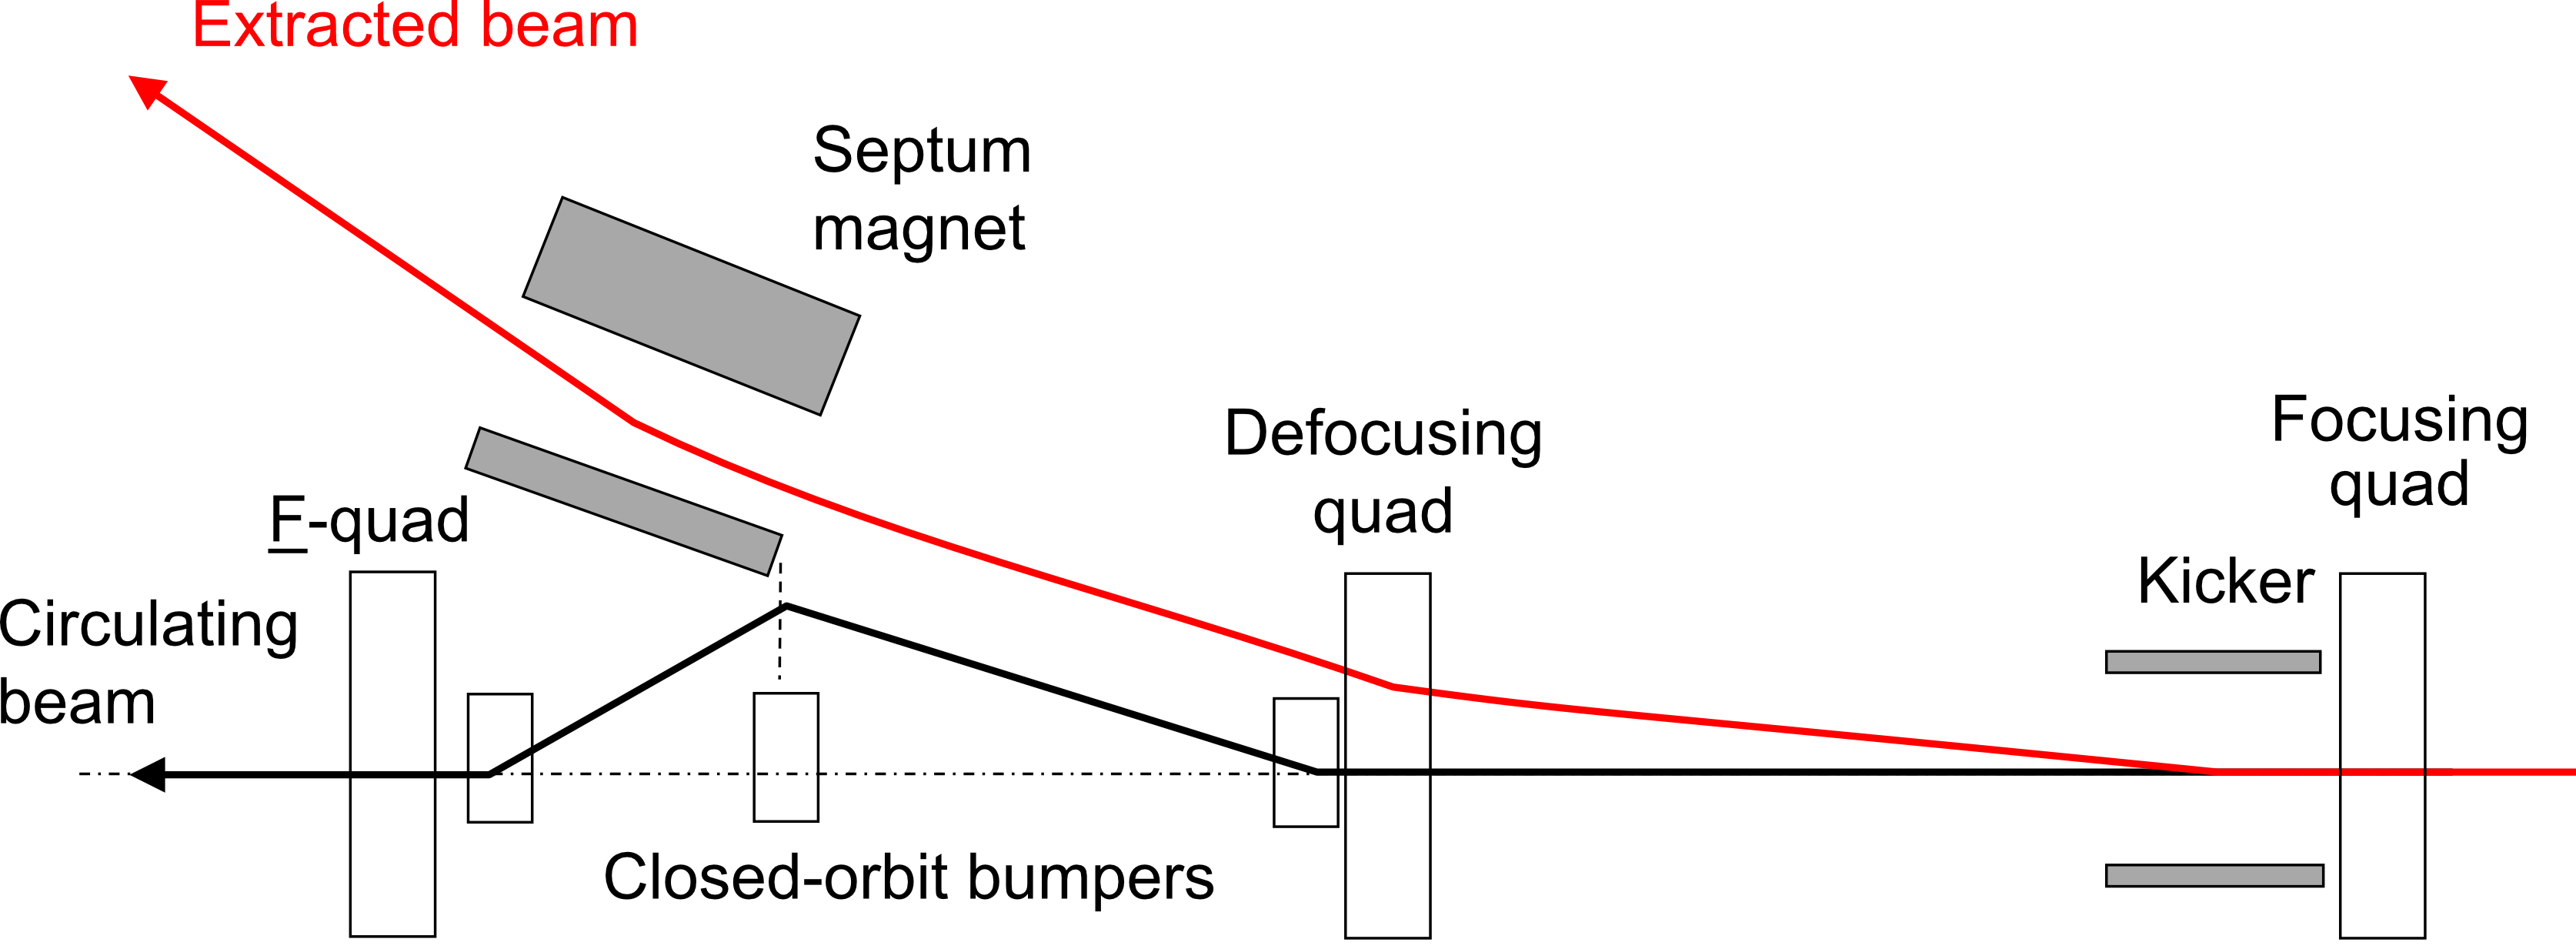
\includegraphics[width=\linewidth]{fast.png}
  \caption{Schematic of a general single-turn fast extraction system~\cite{Fraser:CAS}.}\label{fig:fast_diagram}
\end{figure}

This method of \textbf{\textit{single-turn} fast extraction} (~\autoref{fig:fast_diagram}) is used at two locations in the SPS---Long Straight Sections (LSS) 4 and 6---to fill the two counter-rotating rings in the LHC~\cite{Fraser:CAS}. The PSB uses the same method, but has the added complexity of ``merging'' four seperate stacked rings to one transfer line~\cite{Metzmacher:2061508}. LEIR likewise performs fast extraction~\cite{Ghithan:2017wpd}. The general layout of these systems are shown in~\ref{fig:chain}, where red diamonds mark fast extraction locations. Fast extraction systems are also used at the beam dump facilities at various stages of the accelerator chain to discard the circulating beam at the SPS and LHC.

In accelerator-to-accelerator contexts, the synchronous nature of fast extraction allows particles to remain bunched.~\textbf{Multi-turn fast extraction} extends this benefit, and is performed when filling the SPS for its fixed-target experiments (North Area) from the PS. As the SPS (\qty{6.9}{km}) is almost approximately 11 times longer in circumference than the PS\footnote{The PS is 100 meters across, and therefore $200\pi$\si{m}} (\qty{628}{m}), the entire SPS can be filled by 11 successive extractions of the full PS. This method, coined as \textit{continuous transfer} (CT), introduces the concept of ``shaving'' the beam with an electrostatic septum. In its current implementation in the PS, the beam is bumped similarly to single-turn fast extraction, but is instead forced over the blade of an electrostatic septum (ES), such that a segment the beam is `sliced' off, kicked towards a magnetic septum (MS), and extracted. The remaining beam is kicked back onto its orbit. The next turn, the beam has been ``rotated'' by a quarter turn, and the process repeats, until the finally the remaining core of the beam is bumped directly to the magnetic septum. This provides a spill to the SPS of five bunches over five beam rotations from a single PS bunch.

\begin{figure}[hb]
  \centering
  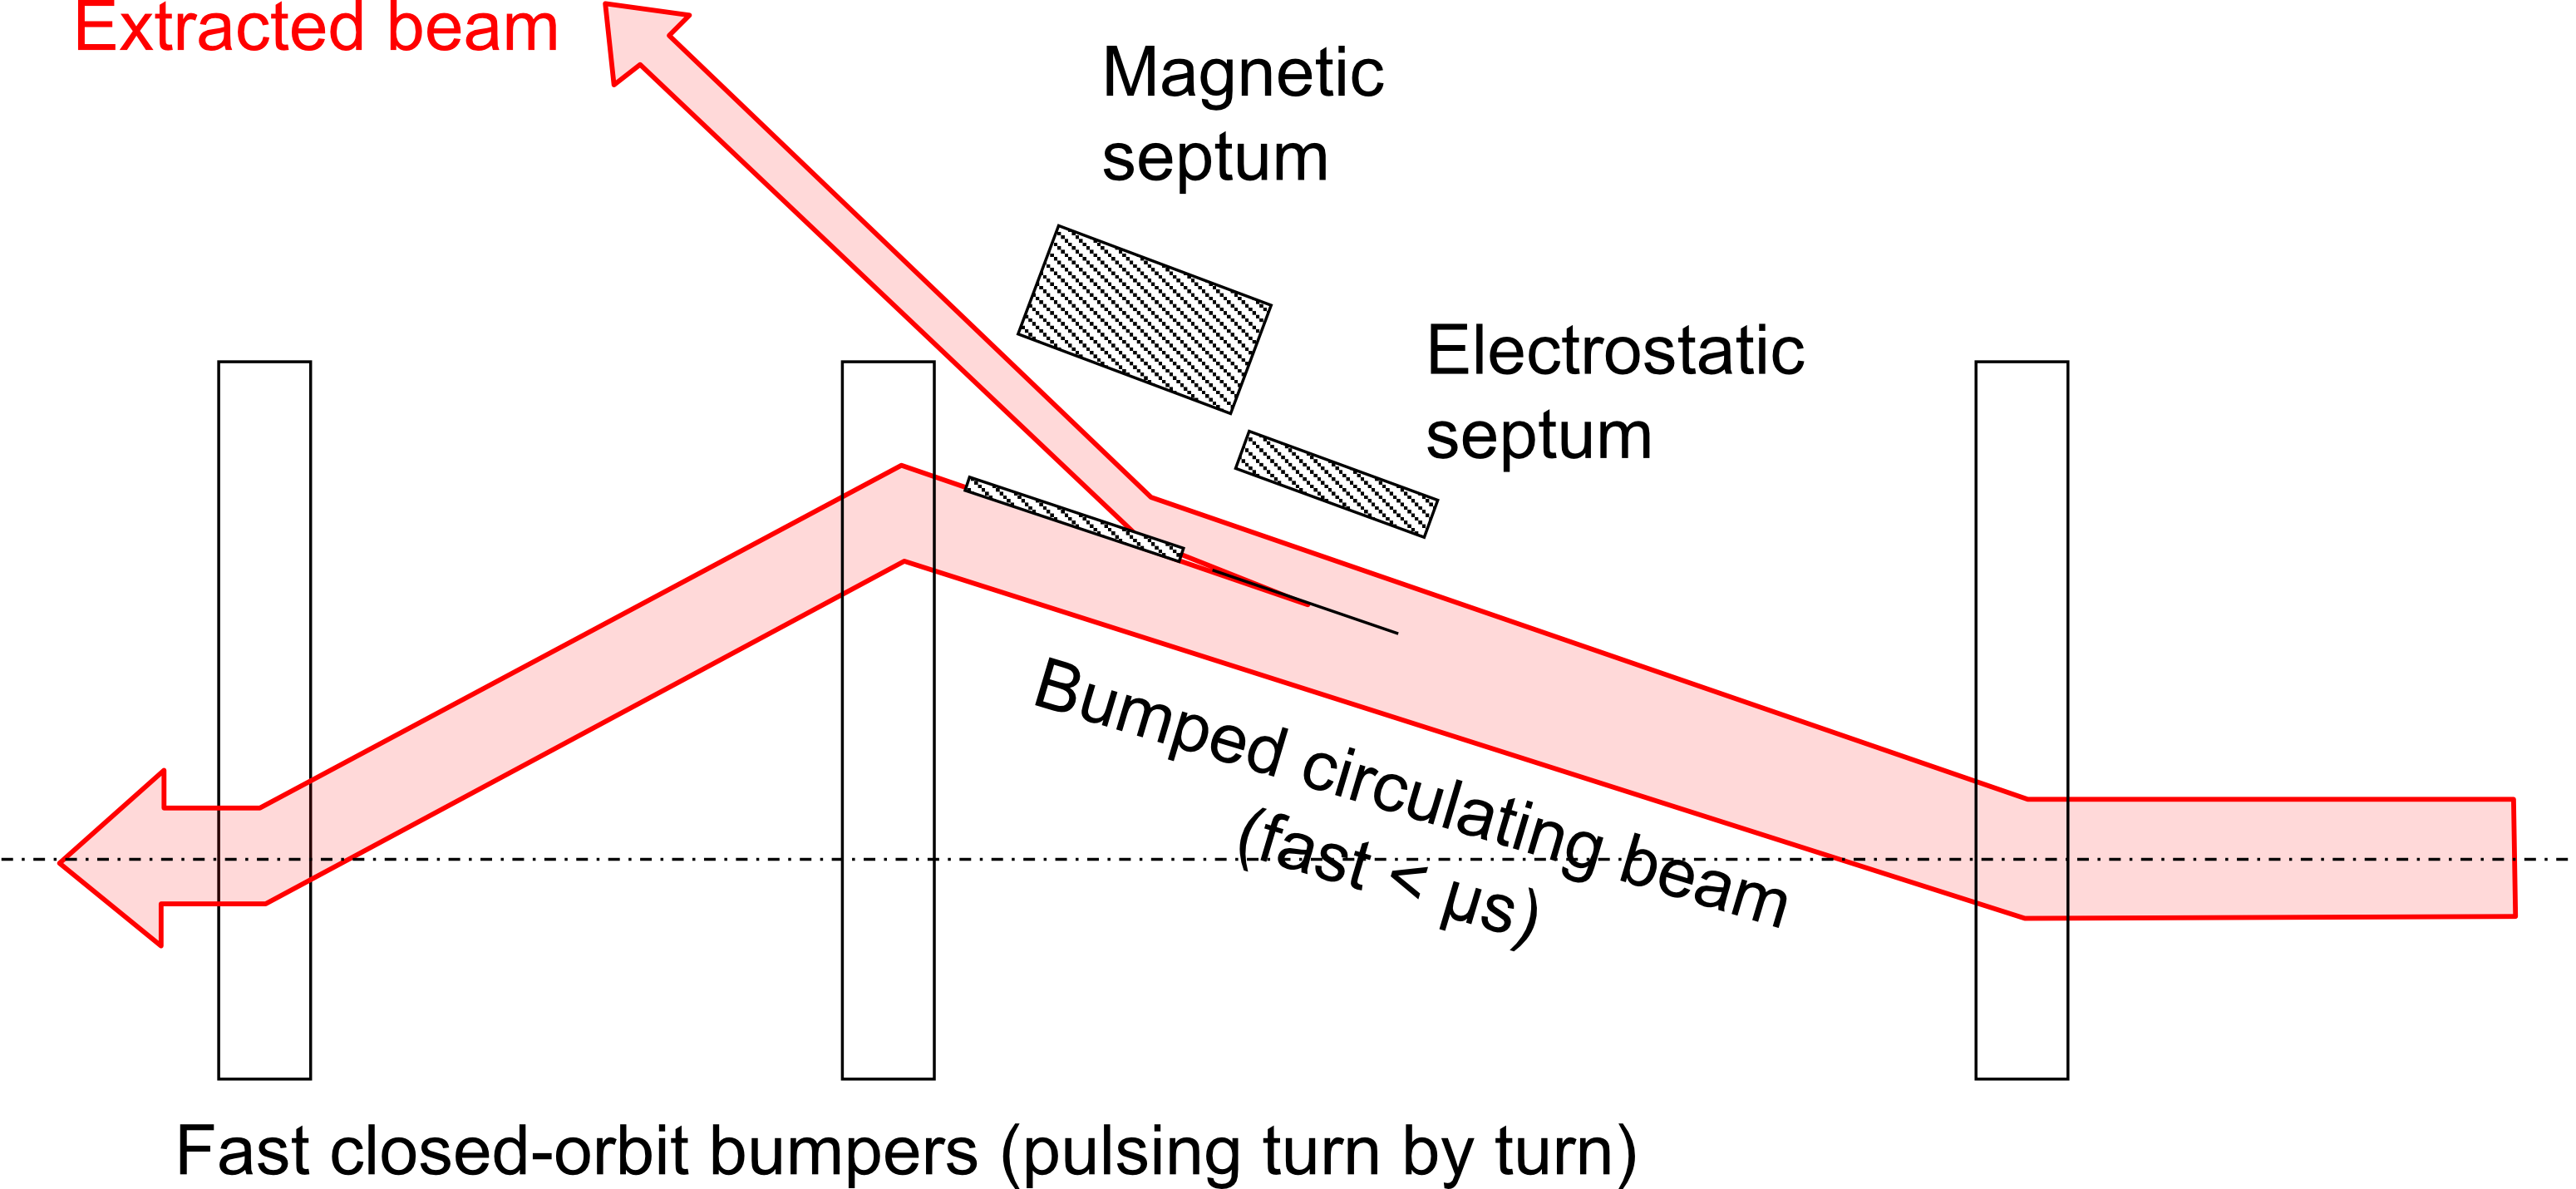
\includegraphics[width=\linewidth]{fastmulti.png}
  \caption{Diagram of a general multi-turn fast extraction system~\cite{Fraser:CAS}.}\label{fig:fast_multi_diagram}
\end{figure}

This method of increasing the spill time is, however, limited by the width of the septum blades. As the amount of beam scraped off per turn decreases, the effect of the particles lost on the septum blade increases. To maintain a reasonable extraction efficiency, the beam size would have to become exponentially large.

For example, if a 50\% extraction efficiency is desired over $10^4$ turns, the beam thickness sliced off by the ES must be the same as the thickness of the blade itself. For the SPS, the ES has blade thickness of \qty{25}{\micro\meter}. The required diameter of the beam, therefore, would be $2\cdot 25\mu m\cdot 10^4 = $ \qty{0.5}{\meter}. This diameter is already lager than the beam pipes, clearly physically impossible.

In order to provide spills over a longer duration, over many thousands of turns, \textit{slow extraction} must be used. 

\subsection{Introduction to Slow Extraction}

\textbf{Slow extraction} instead relies on exploiting resonance of the beam as it oscillates around the orbit of the machine. A full theoretical description of these effects will be detailed in \autoref{chap:theory}, but a brief explanation is offered here: the oscillatory motion of a beam can be controlled such that it returns to the same point along the accelerators circumference with the same oscillation phase. The particles will, therefore, travel through the same field of a magnet, and experience the same force on consecutive turns, rapidly becoming unstable.

This resonant effect is usually carefully avoided in particle accelerators. However, with the right configuration, this amplitude growth can be used alongside an ES to separate particles from their orbit, towards an MS, and into the extraction transfer line. Should the effect be slow enough, a small fraction of particles will reach the MS per turns.

The exploitation of resonance to induce extraction is by no means novel; a method akin to slow extraction was first proposed by J. Tuck and L. Teng in 1951~\cite{Couteur_1951}, and performed by Le Couteur at the Liverpool cyclotron in 1954~\cite{Couteur_1955}. Many such applications of slow extraction exist, using different effects to drive particles into resonance. This thesis will present some of these methods, particularly focussing on Radio-Frequency Knock-Out slow extraction.

Many medical synchrotrons, such as the MedAustron Synchrotron, use slow extraction to deliver beam to patients for ion beam cancer therapy~\cite{ArrutiaSota:2845862}, producing spills of up to \qty{30}{\second} can be produced\footnote{Limited to \qty{10}{\second} for patient treatment}. In human medical applications, safety is paramount. Therefore, the slow extraction process must be fully understood. Ripples in the intensity of beam have to be carefully controlled in order to provide a steady, predictable irradiation dose to patients.

Small medical synchrotrons are simpler\footnote{The PS contains 100 bending magnets along its circumference, as opposed to MedAustron's 16}, newer\footnote{The PS began operation in 1959, and is CERN's oldest accelerator still in operation. MedAustron was first certified in 2016.}, and having a far higher operational availability requirement than research accelerators such as the PS. At CERN's PS, however, that benefit cannot be relied upon. Machine time is in high demand, and studies are time-shared between machine development (MD), fixed-target experimental areas, LHC physics injection, and a wide array of other facilities. 

Simulations can there provide an important tool in understanding slow extraction spills. New methods can be rapidly developed and tested without requiring extensive (and expensive) machine studies, and wide parameter spaces can be explored to construct functional relationships between input parameters and spill output characteristics. 

\section{Modelling Slow Extraction}

\autoref{sec:matrix} will introduce a mathematical model which can be used to numerically calculate particle trajectories in simple machines. However, with even the simplest of accelerators at CERN containing hundreds of components, computational models quickly become necessary. In addition, slow extraction can operate over many more accelerator turns than other processes, such as fast single-turn injection. In the PS, a spill length of \qty{0.5}{\second} would require approximate 230,000 turns. For even a reasonably powerful machine, these computational simulations quickly become time-consuming. 

To aid with the design and construction of CERN's Large Electron-Positron collider (LEP, the predecessor to LHC), the \textit{Methodical Accelerator Design Program} (MAD)~\cite{Iselin:MAD} was developed. This FORTRAN-based scripting tool allowed physicists to define the arrangement and strengths of magnetic elements around an accelerator (the \textit{lattice}), define beam parameters, and calculate the resulting motion of particles (the \textit{optics}). MAD, and its latest version, \verb|MAD-X|, quickly became the \textit{de facto} standard within CERN's beam physics community. However, in the twenty years since the release of \verb|MAD-X|, the landscape of computational accelerator physics has become awash with a wide array of tools, codes, and standards, each with their own specialisations. 

However, newer tools are introducing improvements, such as ``ready-to-go'' compatibility with General-Purpose Graphical Processing Unit (GPGPU) acceleration. GPUs are specialised hardware capable of performing highly optimised matrix and vector calculations. This makes them ideal for the matrix calculations required for particle accelerator simulations. Additionally, \textit{embarassingly parallel}\footnote{A problem which requires minimal no effort to be separated into a large number of independent, concurrently-processed tasks.} can be run on large number of smaller processing platforms, rather than a single large platform. These platforms could be processing units within a GPGPU, or discrete computer host on a batch-processing network.

\chapter{Accelerator Physics Theory}\label{chap:theory}

To construct accurate simulations of slow extraction methods, one must first understand the fundamental theory behind particle motion in a circular accelerator. This chapter will introduce the theory required to understand the motion of particles as they travel through an accelerator, and how such oscillatory motion can be exploited to perform slow extraction~\cite{Wiedemann}.
\section{Single-Particle Transverse Beam Dynamics}

\subsection{Coordinate System}

The coordinate systems used to describe the dynamic motion of particles in an accelerator such as the PS relies on the periodic nature of a circular accelerator. Using a traditional Cartesian coordinate system would quickly introduce complications when describing circular trajectories, and so a local curvilinear coordinate system is used~\cite{BDSIM}.

The basis vectors for this system, $(\hat x, \hat y, \hat s)$, rotate in space as the reference particle moves along the accelerator. The longitudinal vector $\hat s$ is tangent to the particle's orbit, and the $\hat x$ direction is parallel to the radius of the accelerator. The absolute direction of $\hat y$ does not change, but makes one complete rotation in one closed orbit of the reference particle through the accelerator. This system is shown in Figure~\ref{fig:frenet-serret}, along with the radius of the circular trajectory $\rho$, and the angle from the origin $s=0$. 

\begin{figure}[!h]
\begin{center}
\tikzset{every picture/.style={line width=0.75pt}} %set default line width to 0.75pt        

\begin{tikzpicture}[x=0.75pt,y=0.75pt,yscale=-1,xscale=1]

%uncomment if require: \path (0,455); %set diagram left start at 0, and has height of 455

%Shape: Ellipse [id:dp0798878508534051] 
\draw   (142,162.5) .. controls (142,129.09) and (199.08,102) .. (269.5,102) .. controls (339.92,102) and (397,129.09) .. (397,162.5) .. controls (397,195.91) and (339.92,223) .. (269.5,223) .. controls (199.08,223) and (142,195.91) .. (142,162.5) -- cycle ;
%Straight Lines [id:da3917612889933506] 
\draw    (269.5,162.5) -- (269.5,57) ;
\draw [shift={(269.5,55)}, rotate = 90] [color={rgb, 255:red, 0; green, 0; blue, 0 }  ][line width=0.75]    (10.93,-3.29) .. controls (6.95,-1.4) and (3.31,-0.3) .. (0,0) .. controls (3.31,0.3) and (6.95,1.4) .. (10.93,3.29)   ;
%Straight Lines [id:da9587552919771436] 
\draw    (397,162.5) -- (269.5,162.5) ;
%Straight Lines [id:da15722891342539147] 
\draw    (269.5,162.5) -- (322.59,215.59) ;
\draw [shift={(324,217)}, rotate = 225] [color={rgb, 255:red, 0; green, 0; blue, 0 }  ][line width=0.75]    (10.93,-3.29) .. controls (6.95,-1.4) and (3.31,-0.3) .. (0,0) .. controls (3.31,0.3) and (6.95,1.4) .. (10.93,3.29)   ;
%Straight Lines [id:da7846346908558013] 
\draw    (324,217) -- (242.93,235.34) ;
\draw [shift={(240,236)}, rotate = 347.25] [fill={rgb, 255:red, 0; green, 0; blue, 0 }  ][line width=0.08]  [draw opacity=0] (10.72,-5.15) -- (0,0) -- (10.72,5.15) -- (7.12,0) -- cycle    ;
%Straight Lines [id:da569421074096844] 
\draw    (324,217) -- (324,141) ;
\draw [shift={(324,138)}, rotate = 90] [fill={rgb, 255:red, 0; green, 0; blue, 0 }  ][line width=0.08]  [draw opacity=0] (10.72,-5.15) -- (0,0) -- (10.72,5.15) -- (7.12,0) -- cycle    ;
%Straight Lines [id:da7806312488509295] 
\draw    (324,217) -- (345.88,238.88) ;
\draw [shift={(348,241)}, rotate = 225] [fill={rgb, 255:red, 0; green, 0; blue, 0 }  ][line width=0.08]  [draw opacity=0] (10.72,-5.15) -- (0,0) -- (10.72,5.15) -- (7.12,0) -- cycle    ;
%Curve Lines [id:da9180655893242637] 
\draw    (280,173) .. controls (284,177) and (291,162) .. (287,163) ;

% Text Node
\draw (406,153.4) node [anchor=north west][inner sep=0.75pt]    {$s=0$};
% Text Node
\draw (294,166.4) node [anchor=north west][inner sep=0.75pt]    {$\theta $};
% Text Node
\draw (271,177.4) node [anchor=north west][inner sep=0.75pt]    {$\rho $};
% Text Node
\draw (320,113.4) node [anchor=north west][inner sep=0.75pt]    {$\hat{y}$};
% Text Node
\draw (224,230.4) node [anchor=north west][inner sep=0.75pt]    {$\hat{s}$};
% Text Node
\draw (350,244.4) node [anchor=north west][inner sep=0.75pt]    {$\hat{x}$};


\end{tikzpicture}
\end{center}
\caption{The vectors used to define the Frenet-Serret coordinate system.}\label{fig:frenet-serret}
\end{figure}

This coordinate system is known as a {\it Frenet-Serret} coordinate system, and can be rigorously defined by the unit vector {\it tangent} to the curve $\hat T$ (pointing in the direction of motion), the unit vector {\it normal} to the tangent and on the tangential plane $\hat N$, and the binormal unit vector $\hat B$, the cross product of $\hat T$ and $\hat N$. These unit vectors, forming an orthonormal basis spanning $\mathbb{R}^3$ are equal to the vectors $\hat x, \hat y, \hat s$ by:
\begin{equation}
\begin{pmatrix}\hat T\\\hat N\\\hat B \end{pmatrix}=\begin{pmatrix}\hat s\\-\hat x\\\hat y \end{pmatrix}
\end{equation}

The coordinate system $(\hat x, \hat y, \hat s)$ relies on the right-hand chirality (Figure~\ref{fig:rhr}) of the vector cross product for the $\hat x$ vector to point radially outwards from the centre of the machine, the $\hat y$ vector points upwards, and the $\hat s$ vector points in the direction of motion. The direction of $\hat x$ to point outwards from the centre of revolution is chosen as injection and extraction line apertures will therefore be located in the positive $\hat x$.

\begin{figure}[!h]
\begin{center}
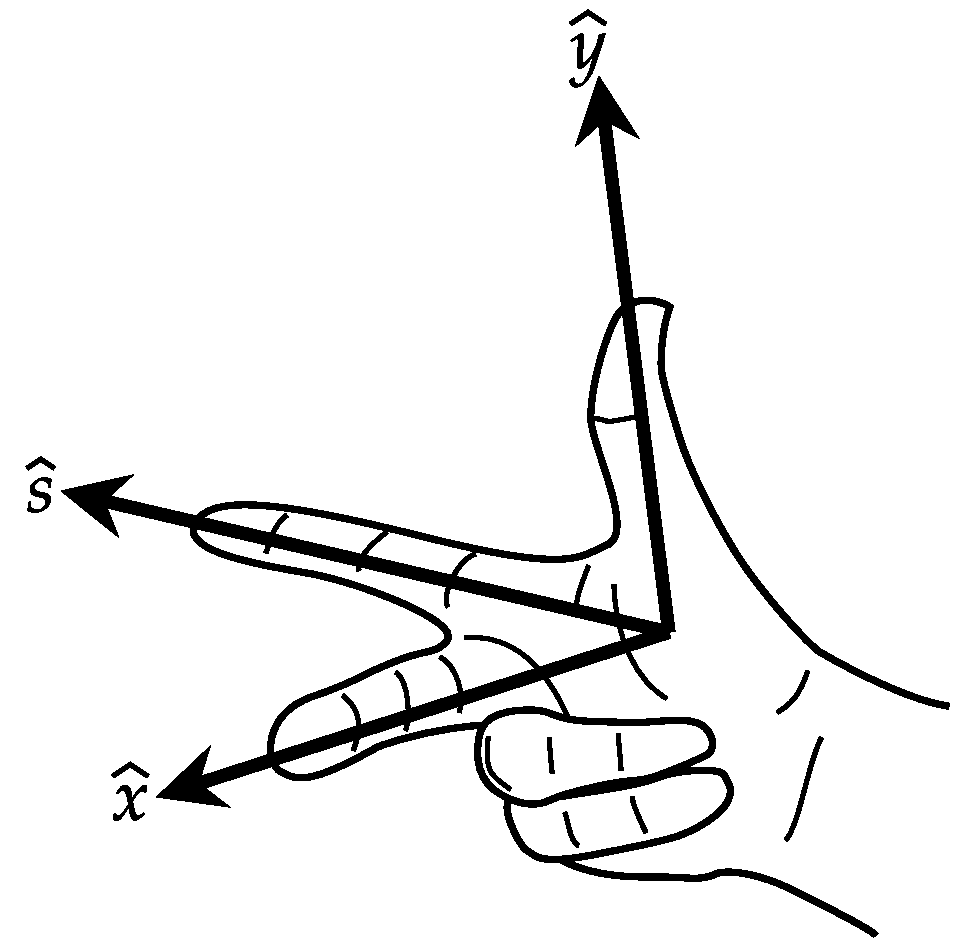
\includegraphics[scale=.25]{rhr.pdf}
\caption{The right-hand chirality rule defining the direction of $\hat x = \hat y \times \hat s$}\label{fig:rhr}
\end{center}
\end{figure}

\subsection{Special Relativity}

The equations of motion in this thesis consider particles moving at extremely high velocity, approaching the speed of light $c$. At CERN, before injection into the PS, particles are accelerated to \qty{2}{\giga\electronvolt}, and reach 94.8\% of the speed of light. At such speeds, relativistic effects are significant.

The Lorentz factor $\gamma$ is defined as the derivative of \textit{coordinate} time $t$ in the relativistic particle's reference frame, with respect to the \textit{proper} or \textit{lab} time $\tau$ in the observer's reference frame. It is calculated as:
\begin{equation}
    \gamma = \frac 1{\sqrt{1-\frac{v^2}{c^2}}}
\end{equation}
Also defined is the $\beta$ factor
\begin{equation}
    \beta = \frac vc
\end{equation}
and the $\alpha$ factor
\begin{equation}
    \alpha = \frac 1\gamma
\end{equation}

For reasons that will become clear in \autoref{subsec:trans_phase_space}, these factors will be referred to as $\alpha_c, \beta_c, \gamma_c$.

One important distinction in a relativistic reference frame is the \textit{invariant} mass $m_0$ versus the \text{relativistic} mass $m$. The invariant mass, or \text{rest} mass of any object is the Newtonian mass measured in its own reference frame. From the \textit{lab} reference frame, this mass is measured as the relativistic mass, defined as
\begin{equation}
    m=\gamma m_0
\end{equation}
This relativistic mass is conserved just the same as rest mass, and follows the $p=mv$ formula the same as in the rest frame. 
The rest \text{energy} $E_0$ and \textit{momentum} $m_0$ are likewise defined in the relativistic frame:
\begin{equation}
    E=\gamma m_0c^2
\end{equation}
\begin{equation}
    p=\gamma m_0v
\end{equation}
For brevity, this report will always assume a relativistic frame, and all mentions of mass $m$, momentum $p$, or energy $E$ should be assumed to be relativistic unless otherwise stated.

\subsection{Particle Variables}

Following the basis vectors defining the coordinate system, the following variables are used to characterise the orbit of particles, dependent on $s$:

\noindent \textbf{In the transverse plane:}
\begin{itemize}
  \item $x(s)$ [m]~---~the particle's horizontal position with respect to the reference orbit.
  \item $y(s)$ [m]~---~the particle's vertical position with respect to the reference orbit.
  \item $x'(s)=\frac{dx}{ds}$ [rad]~---~the particle's horizontal angle with respect to the reference orbit.
  \item $y'(s)=\frac{dy}{ds}$ [rad]~---~the particle's vertical angle with respect to the reference orbit.
\end{itemize}
\textbf{In the longitudinal plane:}
\begin{itemize}
    \item $z=s-s_0$~---~the particle's longitudinal position with respect to the reference particle $s_0$.
    \item $\delta = \Delta p/p_0$~---~the particle's momentum difference with respect to the reference particle $p_0$.
    %\item $t(s)=-c\Delta t$ [m]~---~the particle's arrival delay with respect to the reference orbit, multiplied by the speed of light $c$.
    %\item $p_t(s)=\Delta E/pc$~---~the particle's energy difference, divided by the reference momentum times the speed of light $c$.
\end{itemize}
\item 

These variables provide a 6-tuple fully describing the position of a particle. However, for the remainder of this thesis, the pair of longitudinal variables $(z, \delta)$ will be treated separately to the transverse variable pairs $(x, x')$ and $(y, y')$. This enables a simpler understanding of the effects of beam bending and focussing magnets, as these effects are independent of the longitudinal variables. Conversely, longitudinal beam dynamics requires understanding or RF devices.

\subsection{Design orbit and Dipoles}

An understanding of particle dynamics in an accelerator can be built upon the Lorentz force, describing the force $\vec F$ acting on a charged particle with charge $q$ as it moves through an electric field $\vec E$ and magnetic field $\vec B$ with velocity $\vec v$, given as
\begin{equation}
\vec F_{\text{lorentz}} = q\cdot(\vec E+ \vec v\times\vec B)\label{eq:lorentz}
\end{equation}
This equation can already show why magnetic fields are used in almost all areas of particle acceleration, and not electric fields; a particle with higher velocity $v$ will experience a greater force from a constant magnetic field $\vec B$, whereas the contribution from the electric field $\vec E$ will remain constant.

The other force experienced by a particle in an accelerator is a consequence of conservation of momentum:
%centripetal\footnote{While the coordinate system used allows for a reference frame whose orientation follows the orbit, this frame is not co-moving with the particles, but still fixed in the ``laboratory'' frame---otherwise, complex Lorentz transformations would be required.} force:
\begin{equation}
\vec F_{\text{centrif.}}=\frac{m_0v^2}{\rho}\label{eq:centrifugal}
\end{equation} where $m_0$ is the particle's rest mass, and $\rho$ is the radius of the particle's orbit inside the accelerator.

Equating equations~\ref{eq:centrifugal} and~\ref{eq:lorentz} yields
\begin{equation}
B\rho=\frac pq
\label{eq:brho}
\end{equation}
The quantity $B\rho$ is known as the \textit{magnetic rigidity} of a beam, and defines the bending angle of a particle for a given magnetic field. 

If the relativistic momentum $p=mv$ of the particle is measured in \unit[per-mode = symbol]{\GeV\per\clight\per amu}, the magnetic rigidity can be expressed in Tesla-meters:
\begin{equation}
B\rho \left[\unit{\tesla\meter}\right] = 3.3356\cdot p\left[\unit{\giga\electronvolt\per\clight}\right]
\end{equation} %B\rho\ \left[\unit{\tesla\meter}\right]=\frac pq=\frac AZ\times3.33564\times q\ \left[\unit[per-mode=symbol]{\GeV\per\clight\per\atomicmassunit}\right]
Again referring to~\autoref{eq:lorentz} (with the help of~\autoref{fig:rhr}), a magnetic field pointed vertically upwards (along the $\hat y$ vector) will cause a positively-charged particle with motion along the $\hat s$ vector to experience a bending force along the $-\hat x$ direction (illustrated in~\autoref{fig:dipole}). This formulation, however, only considers a single dipole. In reality, the bending magnet structure of accelerators typically consist of multiple dipoles placed around the ring, their power converters connecting in series. The arrangements of these bending magnets---referred to as Main Units (MU) in the context of the PS---will define the reference\footnote{Sometimes referred to as \textit{design} orbit} orbit in the accelerator.

\begin{figure}[h]
  \centering

  

\tikzset{every picture/.style={line width=0.75pt}} %set default line width to 0.75pt        

\begin{tikzpicture}[x=0.75pt,y=0.75pt,yscale=-1,xscale=1]
%uncomment if require: \path (0,420); %set diagram left start at 0, and has height of 420

%Shape: Rectangle [id:dp3699492063250047] 
\draw   (100,70) -- (250,70) -- (250,130) -- (100,130) -- cycle ;
%Curve Lines [id:da992200965639283] 
\draw [line width=2.25]    (90,100) .. controls (139.78,99.61) and (233.94,90.96) .. (286.81,71.22) ;
\draw [shift={(290,70)}, rotate = 158.46] [color={rgb, 255:red, 0; green, 0; blue, 0 }  ][line width=2.25]    (17.49,-5.26) .. controls (11.12,-2.23) and (5.29,-0.48) .. (0,0) .. controls (5.29,0.48) and (11.12,2.23) .. (17.49,5.26)   ;
%Shape: Rectangle [id:dp8960939916911084] 
\draw   (320,70) -- (390,70) -- (390,130) -- (320,130) -- cycle ;
%Shape: Rectangle [id:dp004915718994831897] 
\draw   (320,60) -- (390,60) -- (390,70) -- (320,70) -- cycle ;
%Shape: Rectangle [id:dp9834216786415646] 
\draw   (320,130) -- (390,130) -- (390,140) -- (320,140) -- cycle ;
%Straight Lines [id:da9215546463069324] 
\draw    (330,80) -- (330,117) ;
\draw [shift={(330,120)}, rotate = 270] [fill={rgb, 255:red, 0; green, 0; blue, 0 }  ][line width=0.08]  [draw opacity=0] (8.93,-4.29) -- (0,0) -- (8.93,4.29) -- cycle    ;
%Straight Lines [id:da4829295704205643] 
\draw    (380,80) -- (380,117) ;
\draw [shift={(380,120)}, rotate = 270] [fill={rgb, 255:red, 0; green, 0; blue, 0 }  ][line width=0.08]  [draw opacity=0] (8.93,-4.29) -- (0,0) -- (8.93,4.29) -- cycle    ;
%Straight Lines [id:da5246257542758568] 
\draw    (355,80) -- (355,117) ;
\draw [shift={(355,120)}, rotate = 270] [fill={rgb, 255:red, 0; green, 0; blue, 0 }  ][line width=0.08]  [draw opacity=0] (8.93,-4.29) -- (0,0) -- (8.93,4.29) -- cycle    ;
%Straight Lines [id:da3445329346880859] 
\draw  [dash pattern={on 4.5pt off 4.5pt}]  (90,100) -- (290,100) ;
%Straight Lines [id:da3150179528223387] 
\draw    (290,100) -- (290,73) ;
\draw [shift={(290,70)}, rotate = 90] [fill={rgb, 255:red, 0; green, 0; blue, 0 }  ][line width=0.08]  [draw opacity=0] (8.93,-4.29) -- (0,0) -- (8.93,4.29) -- cycle    ;
%Flowchart: Summing Junction [id:dp7903638162414015] 
\draw   (107,114.9) .. controls (107,110.43) and (110.63,106.8) .. (115.1,106.8) .. controls (119.57,106.8) and (123.2,110.43) .. (123.2,114.9) .. controls (123.2,119.37) and (119.57,123) .. (115.1,123) .. controls (110.63,123) and (107,119.37) .. (107,114.9) -- cycle ; \draw   (109.37,109.17) -- (120.83,120.63) ; \draw   (120.83,109.17) -- (109.37,120.63) ;

% Text Node
\draw (334.5,42) node [anchor=north west][inner sep=0.75pt]   [align=left] {\begin{minipage}[lt]{27.66pt}\setlength\topsep{0pt}
\begin{center}
North
\end{center}

\end{minipage}};
% Text Node
\draw (336,141) node [anchor=north west][inner sep=0.75pt]   [align=left] {\begin{minipage}[lt]{29.38pt}\setlength\topsep{0pt}
\begin{center}
South
\end{center}

\end{minipage}};
% Text Node
\draw (361,84) node [anchor=north west][inner sep=0.75pt]   [align=left] {\begin{minipage}[lt]{9.78pt}\setlength\topsep{0pt}
\begin{center}
$\displaystyle \vec{B}$
\end{center}

\end{minipage}};
% Text Node
\draw (289,48) node [anchor=north west][inner sep=0.75pt]   [align=left] {\begin{minipage}[lt]{8.67pt}\setlength\topsep{0pt}
\begin{center}
$\displaystyle \vec{v}$
\end{center}

\end{minipage}};
% Text Node
\draw (292,73) node [anchor=north west][inner sep=0.75pt]   [align=left] {\begin{minipage}[lt]{9.14pt}\setlength\topsep{0pt}
\begin{center}
$\displaystyle \vec{F}$
\end{center}

\end{minipage}};
% Text Node
\draw (153,42) node [anchor=north west][inner sep=0.75pt]   [align=left] {\begin{minipage}[lt]{31.64pt}\setlength\topsep{0pt}
\begin{center}
Dipole
\end{center}

\end{minipage}};
% Text Node
\draw (123.5,171) node [anchor=north west][inner sep=0.75pt]   [align=left] {Top-down View};
% Text Node
\draw (311,172) node [anchor=north west][inner sep=0.75pt]   [align=left] {Front-on View};
% Text Node
\draw (128,101) node [anchor=north west][inner sep=0.75pt]   [align=left] {\begin{minipage}[lt]{9.78pt}\setlength\topsep{0pt}
\begin{center}
$\displaystyle \vec{B}$
\end{center}

\end{minipage}};


\end{tikzpicture}
  
  \caption{A dipole magnet, showing the direction of the magnetic field $\vec B$ into the page (left, upwards in front-on view), the current velocity of a positively charged particle $\vec v$, and the Lorentz force $\vec F$, as calculated by $\vec F=q\vec v\times\vec B$}\label{fig:dipole}
\end{figure}

If $\alpha$ is the bending angle of a single MU, then $\alpha$ can be related to the magnetic rigidity by
\begin{equation}
\alpha=\frac{ds}\rho=\frac{B\ ds}{B\rho}
\end{equation}
Integrating this over all magnets in the ring, therefore, must be equal to one full revolution, $2\pi$
\begin{equation}
\frac{\int B\ ds}{B\rho}\equiv2\pi
\end{equation}

This provides one of the first key insights which is not obvious at first---that ``circular'' accelerators are in fact more complex shapes, with bending magnets at each vertex, and a \textit{drift} (accelerator sections without any significant electromagnetic field) or other non-bending multipole magnet at each side: in the case of the LHC, 1,232 dipole magnets are used to keep the beam on it's circular path; in the PS---100.

\subsection{Focussing and Multipoles}

\begin{figure}[h]
\centering
\tikzset{every picture/.style={line width=0.75pt}} %set default line width to 0.75pt        
\begin{tikzpicture}[x=0.75pt,y=0.75pt,yscale=-1,xscale=1]
%uncomment if require: \path (0,556); %set diagram left start at 0, and has height of 556
%Curve Lines [id:da992200965639283] 
\draw [line width=2.25]    (191.6,294.6) .. controls (253.97,235.2) and (403.57,229.71) .. (486.12,291.7) ;
\draw [shift={(488.6,293.6)}, rotate = 217.97] [color={rgb, 255:red, 0; green, 0; blue, 0 }  ][line width=2.25]    (17.49,-5.26) .. controls (11.12,-2.23) and (5.29,-0.48) .. (0,0) .. controls (5.29,0.48) and (11.12,2.23) .. (17.49,5.26)   ;
%Shape: Trapezoid [id:dp1586228139836543] 
\draw   (420,190) -- (371.6,320) -- (288.4,320) -- (240,190) -- cycle ;
%Flowchart: Summing Junction [id:dp5579894688888893] 
\draw   (251,205) .. controls (251,201.13) and (254.13,198) .. (258,198) .. controls (261.87,198) and (265,201.13) .. (265,205) .. controls (265,208.87) and (261.87,212) .. (258,212) .. controls (254.13,212) and (251,208.87) .. (251,205) -- cycle ; \draw   (253.05,200.05) -- (262.95,209.95) ; \draw   (262.95,200.05) -- (253.05,209.95) ;
%Straight Lines [id:da5730652497322037] 
\draw  [dash pattern={on 4.5pt off 4.5pt}]  (288.4,320) -- (329.6,434.6) ;
%Straight Lines [id:da7372483569632045] 
\draw  [dash pattern={on 4.5pt off 4.5pt}]  (371.6,320) -- (329.6,434.6) ;
%Curve Lines [id:da13311837170498553] 
\draw [line width=2.25]    (265.6,255.6) .. controls (329.95,242.73) and (391.36,225.94) .. (497.37,236.28) ;
\draw [shift={(500.6,236.6)}, rotate = 185.82] [color={rgb, 255:red, 0; green, 0; blue, 0 }  ][line width=2.25]    (17.49,-5.26) .. controls (11.12,-2.23) and (5.29,-0.48) .. (0,0) .. controls (5.29,0.48) and (11.12,2.23) .. (17.49,5.26)   ;
%Straight Lines [id:da8412635645751751] 
\draw    (500.19,238.56) -- (489.01,291.64) ;
\draw [shift={(488.6,293.6)}, rotate = 281.89] [color={rgb, 255:red, 0; green, 0; blue, 0 }  ][line width=0.75]    (10.93,-3.29) .. controls (6.95,-1.4) and (3.31,-0.3) .. (0,0) .. controls (3.31,0.3) and (6.95,1.4) .. (10.93,3.29)   ;
\draw [shift={(500.6,236.6)}, rotate = 101.89] [color={rgb, 255:red, 0; green, 0; blue, 0 }  ][line width=0.75]    (10.93,-3.29) .. controls (6.95,-1.4) and (3.31,-0.3) .. (0,0) .. controls (3.31,0.3) and (6.95,1.4) .. (10.93,3.29)   ;

% Text Node
\draw (481,302) node [anchor=north west][inner sep=0.75pt]   [align=left] {$\displaystyle p_{0}$};
% Text Node
\draw (267,193) node [anchor=north west][inner sep=0.75pt]   [align=left] {$\displaystyle \vec{B}$};
% Text Node
\draw (491,206) node [anchor=north west][inner sep=0.75pt]   [align=left] {$\displaystyle p_{0} +\delta p$};
% Text Node
\draw (324,383) node [anchor=north west][inner sep=0.75pt]   [align=left] {$\displaystyle \theta $};
% Text Node
\draw (502,254) node [anchor=north west][inner sep=0.75pt]   [align=left] {$\displaystyle D( s) \delta $};

\end{tikzpicture}
\caption{A top-down diagram of a sector dipole illustrating how small changes in the beam's momentum ($\delta = (p-p_0)/p_0$), lead to significant changes in the bending effect of a dipole.}
\label{fig:dipole_error}
\end{figure}

\autoref{fig:dipole_error} illustrates the need for corrective elements in the beamline. If a particle is displaced slightly from the design orbit ($x=0$) or has a variation in momentum ($\delta$) before a dipole element (marked with a downwards magnetic field $\vec B$), the bending effect will differ, and the particle will be displaced from the design orbit after the dipole. This difference in bending effect is known as \textit{dispersion}, and will be analysed in~\autoref{sec:transdisp}.

To correct for this, synchrotrons use quadrupole elements to ``focus'' the beam in one transverse plane. An arrangement of four magnetic poles creates a field stronger at higher $|x|$ displacement, causing particles to be pulled back towards the design orbit. However, particles off-axis in the other transverse plane will be pushed further off-axis. To correct for this, a second quadrupole is placed further along in the beamline, with the magnetic poles arranged in the opposite orientation. This arrangement, known as a FODO lattice, is shown in \autoref{fig:quadrupole} (right).

\begin{figure}
\centering
\tikzset{every picture/.style={line width=0.75pt}} %set default line width to 0.75pt        
\begin{tikzpicture}[x=0.75pt,y=0.75pt,yscale=-1,xscale=1]
%uncomment if require: \path (0,300); %set diagram left start at 0, and has height of 300
%Shape: Rectangle [id:dp16895106513799774] 
\draw   (165.86,51.72) -- (208.28,94.14) -- (194.14,108.28) -- (151.72,65.86) -- cycle ;
%Shape: Rectangle [id:dp7670602245044726] 
\draw   (75.86,141.72) -- (118.28,184.14) -- (104.14,198.28) -- (61.72,155.86) -- cycle ;
%Shape: Rectangle [id:dp12217894090817283] 
\draw   (208.28,155.86) -- (165.86,198.28) -- (151.72,184.14) -- (194.14,141.72) -- cycle ;
%Shape: Rectangle [id:dp07589692725962705] 
\draw   (118.28,65.86) -- (75.86,108.28) -- (61.72,94.14) -- (104.14,51.72) -- cycle ;
%Curve Lines [id:da018342825147440456] 
\draw    (80,100) .. controls (88.56,113.58) and (88.29,136.15) .. (81.62,147.61) ;
\draw [shift={(80,150)}, rotate = 308.25] [fill={rgb, 255:red, 0; green, 0; blue, 0 }  ][line width=0.08]  [draw opacity=0] (8.93,-4.29) -- (0,0) -- (8.93,4.29) -- cycle    ;
%Curve Lines [id:da03259735785014195] 
\draw    (110,70) .. controls (123.98,76.99) and (145.42,74.17) .. (157.17,70.87) ;
\draw [shift={(160,70)}, rotate = 161.57] [fill={rgb, 255:red, 0; green, 0; blue, 0 }  ][line width=0.08]  [draw opacity=0] (8.93,-4.29) -- (0,0) -- (8.93,4.29) -- cycle    ;
%Curve Lines [id:da729590423325807] 
\draw    (89.2,96.6) .. controls (103.87,116.48) and (102.52,130.21) .. (90.54,151.28) ;
\draw [shift={(89.2,153.6)}, rotate = 300.51] [fill={rgb, 255:red, 0; green, 0; blue, 0 }  ][line width=0.08]  [draw opacity=0] (8.93,-4.29) -- (0,0) -- (8.93,4.29) -- cycle    ;
%Curve Lines [id:da08909499648653463] 
\draw    (96.2,89.6) .. controls (115.5,106) and (114.31,137.31) .. (98.03,158.35) ;
\draw [shift={(96.2,160.6)}, rotate = 310.6] [fill={rgb, 255:red, 0; green, 0; blue, 0 }  ][line width=0.08]  [draw opacity=0] (8.93,-4.29) -- (0,0) -- (8.93,4.29) -- cycle    ;
%Curve Lines [id:da4406082857174254] 
\draw    (184.42,100.04) .. controls (170.84,119.33) and (173.24,133.1) .. (186.2,154.6) ;
\draw [shift={(186.2,97.6)}, rotate = 127.04] [fill={rgb, 255:red, 0; green, 0; blue, 0 }  ][line width=0.08]  [draw opacity=0] (8.93,-4.29) -- (0,0) -- (8.93,4.29) -- cycle    ;
%Curve Lines [id:da930807564323026] 
\draw    (176.7,92.71) .. controls (158.78,110.22) and (161.37,141.44) .. (179.04,161.6) ;
\draw [shift={(179.04,90.6)}, rotate = 140.27] [fill={rgb, 255:red, 0; green, 0; blue, 0 }  ][line width=0.08]  [draw opacity=0] (8.93,-4.29) -- (0,0) -- (8.93,4.29) -- cycle    ;
%Curve Lines [id:da5120218997402282] 
\draw    (111.04,172.69) .. controls (130.22,159.71) and (143.94,162.15) .. (165.29,174.83) ;
\draw [shift={(108.29,174.63)}, rotate = 323.78] [fill={rgb, 255:red, 0; green, 0; blue, 0 }  ][line width=0.08]  [draw opacity=0] (8.93,-4.29) -- (0,0) -- (8.93,4.29) -- cycle    ;
%Curve Lines [id:da8390452720928254] 
\draw    (103.45,165.31) .. controls (121.22,147.77) and (154.92,149.37) .. (172.32,167.85) ;
\draw [shift={(101.32,167.61)}, rotate = 310.56] [fill={rgb, 255:red, 0; green, 0; blue, 0 }  ][line width=0.08]  [draw opacity=0] (8.93,-4.29) -- (0,0) -- (8.93,4.29) -- cycle    ;
%Curve Lines [id:da6235876089908017] 
\draw    (113.26,178.83) .. controls (130.38,174.41) and (148.87,172.99) .. (160.29,179.63) ;
\draw [shift={(110.29,179.63)}, rotate = 344.31] [fill={rgb, 255:red, 0; green, 0; blue, 0 }  ][line width=0.08]  [draw opacity=0] (8.93,-4.29) -- (0,0) -- (8.93,4.29) -- cycle    ;
%Curve Lines [id:da24851523512173146] 
\draw    (106.29,76.02) .. controls (126.22,89.93) and (139.95,88.6) .. (160.98,77.12) ;
\draw [shift={(163.29,75.83)}, rotate = 150.49] [fill={rgb, 255:red, 0; green, 0; blue, 0 }  ][line width=0.08]  [draw opacity=0] (8.93,-4.29) -- (0,0) -- (8.93,4.29) -- cycle    ;
%Curve Lines [id:da9241759818534776] 
\draw    (99.32,82.71) .. controls (115.79,101.04) and (149.72,100.86) .. (168.35,84.34) ;
\draw [shift={(170.32,82.48)}, rotate = 134.64] [fill={rgb, 255:red, 0; green, 0; blue, 0 }  ][line width=0.08]  [draw opacity=0] (8.93,-4.29) -- (0,0) -- (8.93,4.29) -- cycle    ;
%Curve Lines [id:da909413050316068] 
\draw    (191.13,103.88) .. controls (185.3,123.95) and (186.46,138.2) .. (192,151) ;
\draw [shift={(192,101)}, rotate = 107.47] [fill={rgb, 255:red, 0; green, 0; blue, 0 }  ][line width=0.08]  [draw opacity=0] (8.93,-4.29) -- (0,0) -- (8.93,4.29) -- cycle    ;
%Straight Lines [id:da22347636828081718] 
\draw  [dash pattern={on 4.5pt off 4.5pt}]  (52,124.8) -- (128,124.8) ;
\draw [shift={(130,124.8)}, rotate = 180] [color={rgb, 255:red, 0; green, 0; blue, 0 }  ][line width=0.75]    (10.93,-3.29) .. controls (6.95,-1.4) and (3.31,-0.3) .. (0,0) .. controls (3.31,0.3) and (6.95,1.4) .. (10.93,3.29)   ;
%Straight Lines [id:da5667501984477679] 
\draw  [dash pattern={on 4.5pt off 4.5pt}]  (142,124.8) -- (162.2,124.8) -- (218,124.8) ;
\draw [shift={(140,124.8)}, rotate = 0] [color={rgb, 255:red, 0; green, 0; blue, 0 }  ][line width=0.75]    (10.93,-3.29) .. controls (6.95,-1.4) and (3.31,-0.3) .. (0,0) .. controls (3.31,0.3) and (6.95,1.4) .. (10.93,3.29)   ;
%Straight Lines [id:da690213494533449] 
\draw  [dash pattern={on 4.5pt off 4.5pt}]  (135,119.8) -- (135,46.6) ;
\draw [shift={(135,44.6)}, rotate = 90] [color={rgb, 255:red, 0; green, 0; blue, 0 }  ][line width=0.75]    (10.93,-3.29) .. controls (6.95,-1.4) and (3.31,-0.3) .. (0,0) .. controls (3.31,0.3) and (6.95,1.4) .. (10.93,3.29)   ;
%Straight Lines [id:da4326059970165157] 
\draw  [dash pattern={on 4.5pt off 4.5pt}]  (135,128.8) -- (135,207.6) ;
\draw [shift={(135,209.6)}, rotate = 270] [color={rgb, 255:red, 0; green, 0; blue, 0 }  ][line width=0.75]    (10.93,-3.29) .. controls (6.95,-1.4) and (3.31,-0.3) .. (0,0) .. controls (3.31,0.3) and (6.95,1.4) .. (10.93,3.29)   ;
%Shape: Ellipse [id:dp34626752560776697] 
\draw   (340.2,124) .. controls (340.2,104.12) and (344.63,88) .. (350.1,88) .. controls (355.57,88) and (360,104.12) .. (360,124) .. controls (360,143.88) and (355.57,160) .. (350.1,160) .. controls (344.63,160) and (340.2,143.88) .. (340.2,124) -- cycle ;
%Straight Lines [id:da6277807791700993] 
\draw [line width=2.25]    (350,100) -- (526.15,148.93) ;
\draw [shift={(530,150)}, rotate = 195.52] [color={rgb, 255:red, 0; green, 0; blue, 0 }  ][line width=2.25]    (17.49,-5.26) .. controls (11.12,-2.23) and (5.29,-0.48) .. (0,0) .. controls (5.29,0.48) and (11.12,2.23) .. (17.49,5.26)   ;
%Shape: Path Data [id:dp6636836986240371] 
\draw   (430,160) .. controls (432.76,160) and (435,144.33) .. (435,125) .. controls (435,105.67) and (432.76,90) .. (430,90) -- (450,90) .. controls (447.24,90) and (445,105.67) .. (445,125) .. controls (445,144.33) and (447.24,160) .. (450,160) -- (430,160) -- cycle ;
%Shape: Ellipse [id:dp8228024181704114] 
\draw   (520,124) .. controls (520,104.12) and (524.43,88) .. (529.9,88) .. controls (535.37,88) and (539.8,104.12) .. (539.8,124) .. controls (539.8,143.88) and (535.37,160) .. (529.9,160) .. controls (524.43,160) and (520,143.88) .. (520,124) -- cycle ;
%Straight Lines [id:da023007468461673675] 
\draw [line width=2.25]    (320,110) -- (346.21,101.26) ;
\draw [shift={(350,100)}, rotate = 161.57] [color={rgb, 255:red, 0; green, 0; blue, 0 }  ][line width=2.25]    (17.49,-5.26) .. controls (11.12,-2.23) and (5.29,-0.48) .. (0,0) .. controls (5.29,0.48) and (11.12,2.23) .. (17.49,5.26)   ;
%Straight Lines [id:da4640302291959706] 
\draw [line width=2.25]    (530,150) -- (556.21,141.26) ;
\draw [shift={(560,140)}, rotate = 161.57] [color={rgb, 255:red, 0; green, 0; blue, 0 }  ][line width=2.25]    (17.49,-5.26) .. controls (11.12,-2.23) and (5.29,-0.48) .. (0,0) .. controls (5.29,0.48) and (11.12,2.23) .. (17.49,5.26)   ;
%Straight Lines [id:da879655645129539] 
\draw  [dash pattern={on 4.5pt off 4.5pt}]  (312.8,125) -- (568.8,125) ;

% Text Node
\draw (84,72) node [anchor=north west][inner sep=0.75pt]   [align=left] {N};
% Text Node
\draw (175,162) node [anchor=north west][inner sep=0.75pt]   [align=left] {N};
% Text Node
\draw (175,71) node [anchor=north west][inner sep=0.75pt]   [align=left] {S};
% Text Node
\draw (85,163) node [anchor=north west][inner sep=0.75pt]   [align=left] {S};
% Text Node
\draw (223,111) node [anchor=north west][inner sep=0.75pt]   [align=left] {$\displaystyle \vec{F}$};
% Text Node
\draw (331,62) node [anchor=north west][inner sep=0.75pt]   [align=left] {Focus};
% Text Node
\draw (412,62) node [anchor=north west][inner sep=0.75pt]   [align=left] {Defocus};
% Text Node
\draw (511,62) node [anchor=north west][inner sep=0.75pt]   [align=left] {Focus};


\end{tikzpicture}
\caption{Diagram (left) showing the field of a \textit{normal} oriented quadrupole, providing focussing in $x$ but defocussing in $y$. The force experienced by a positively-charged particle is shown as dashed arrows. Right-hand diagram illustrates a FODO cell.}
\label{fig:quadrupole}
\end{figure}


% \begin{figure}
%   \centering
%   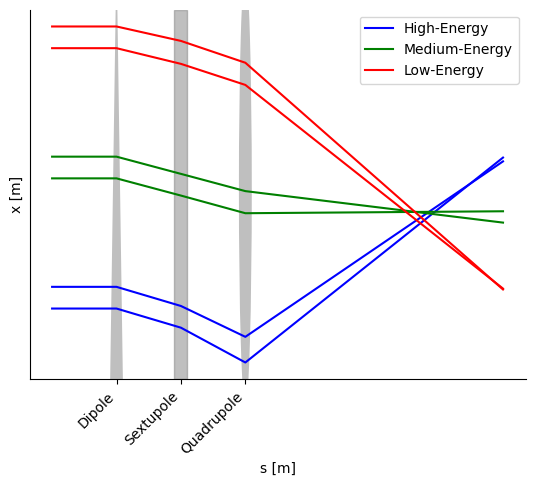
\includegraphics[width=0.6\linewidth]{optics-example.png}
%   \caption{A diagram showing how Dipoles, Quadrupoles, and Sextupoles are used together to create the desired beam dynamics for particles with different energies.}\label{fig:optics}
% \end{figure}

Sextupoles---third order magnets---provide additional correction to the beam. Depicted in~\autoref{fig:sextupole}, these can be understood by expanding on the optical analogy used thus far, where the Dipole takes the role of a prism, bending the light. As with prisms, beams with higher energy are bent less than low energy, and so the component wavelengths (or energies) in the beam beam are dispersed. The sextupole is analogous to an aspherical element, correcting for chromatic aberration introduced by the focussing quadrupole. Again, as with its optical analogue---a focussing lens---the quadrupole has shorter focal length for higher energy particles. The sextupole acts as a focussing lens at high energy and diverging lens at low energy, correcting for this chromatic effect.

\begin{figure}
    \centering
\tikzset{every picture/.style={line width=0.75pt}} %set default line width to 0.75pt        
\begin{tikzpicture}[x=0.75pt,y=0.75pt,yscale=-1,xscale=1]
%uncomment if require: \path (0,300); %set diagram left start at 0, and has height of 300

%Curve Lines [id:da930807564323026] 
\draw    (432.99,71.24) .. controls (448.36,77.05) and (460.19,72.18) .. (460,50) ;
\draw [shift={(430,70)}, rotate = 24.34] [fill={rgb, 255:red, 0; green, 0; blue, 0 }  ][line width=0.08]  [draw opacity=0] (8.93,-4.29) -- (0,0) -- (8.93,4.29) -- cycle    ;
%Shape: Rectangle [id:dp013004832065804717] 
\draw   (440,30.17) -- (501.96,30.17) -- (501.96,50.83) -- (440,50.83) -- cycle ;

%Shape: Rectangle [id:dp0046311061182631175] 
\draw   (439.17,157.34) -- (501.13,157.34) -- (501.13,177.99) -- (439.17,177.99) -- cycle ;
%Shape: Rectangle [id:dp39817022789023415] 
\draw   (519.02,40) -- (550,93.66) -- (532.11,103.99) -- (501.13,50.33) -- cycle ;
%Shape: Rectangle [id:dp567141395429372] 
\draw   (550,114.34) -- (519.02,168) -- (501.13,157.67) -- (532.11,104.01) -- cycle ;
%Shape: Rectangle [id:dp6785221133592134] 
\draw   (421.28,167.66) -- (390.3,114) -- (408.19,103.67) -- (439.17,157.34) -- cycle ;
%Shape: Rectangle [id:dp9504575123901953] 
\draw   (440,50.83) -- (409.02,104.49) -- (391.13,94.16) -- (422.11,40.5) -- cycle ;
%Curve Lines [id:da6493708735943702] 
\draw    (507.27,71.56) .. controls (493.1,78.82) and (480.19,72.18) .. (480,50) ;
\draw [shift={(510,70)}, rotate = 147.72] [fill={rgb, 255:red, 0; green, 0; blue, 0 }  ][line width=0.08]  [draw opacity=0] (8.93,-4.29) -- (0,0) -- (8.93,4.29) -- cycle    ;
%Curve Lines [id:da44762366064755477] 
\draw    (422.66,91.45) .. controls (438.47,100.7) and (435.01,111.07) .. (420,120) ;
\draw [shift={(420,90)}, rotate = 27.05] [fill={rgb, 255:red, 0; green, 0; blue, 0 }  ][line width=0.08]  [draw opacity=0] (8.93,-4.29) -- (0,0) -- (8.93,4.29) -- cycle    ;
%Curve Lines [id:da5120715001347833] 
\draw    (460,156.95) .. controls (459.28,136.09) and (443.18,131.02) .. (430,140) ;
\draw [shift={(460,160)}, rotate = 271.96] [fill={rgb, 255:red, 0; green, 0; blue, 0 }  ][line width=0.08]  [draw opacity=0] (8.93,-4.29) -- (0,0) -- (8.93,4.29) -- cycle    ;
%Curve Lines [id:da6084093795236516] 
\draw    (480.19,156.95) .. controls (482.15,136.18) and (496.44,131.98) .. (510,140) ;
\draw [shift={(480,160)}, rotate = 271.96] [fill={rgb, 255:red, 0; green, 0; blue, 0 }  ][line width=0.08]  [draw opacity=0] (8.93,-4.29) -- (0,0) -- (8.93,4.29) -- cycle    ;
%Curve Lines [id:da5911117332573328] 
\draw    (517.64,91.9) .. controls (504.95,102.7) and (506.58,112.06) .. (520,120) ;
\draw [shift={(520,90)}, rotate = 142.65] [fill={rgb, 255:red, 0; green, 0; blue, 0 }  ][line width=0.08]  [draw opacity=0] (8.93,-4.29) -- (0,0) -- (8.93,4.29) -- cycle    ;
%Curve Lines [id:da5901005430959838] 
\draw    (426.74,80.35) .. controls (444.51,88.37) and (469.61,85.37) .. (469.8,50.6) ;
\draw [shift={(424,79)}, rotate = 28.34] [fill={rgb, 255:red, 0; green, 0; blue, 0 }  ][line width=0.08]  [draw opacity=0] (8.93,-4.29) -- (0,0) -- (8.93,4.29) -- cycle    ;
%Curve Lines [id:da8751448369534596] 
\draw    (516.87,81.2) .. controls (491.9,90.27) and (469.61,85.74) .. (469.8,50.6) ;
\draw [shift={(520,80)}, rotate = 157.97] [fill={rgb, 255:red, 0; green, 0; blue, 0 }  ][line width=0.08]  [draw opacity=0] (8.93,-4.29) -- (0,0) -- (8.93,4.29) -- cycle    ;
%Curve Lines [id:da9461247171380158] 
\draw    (516.97,81.35) .. controls (493.68,92.74) and (492.8,118.16) .. (516.8,131.6) ;
\draw [shift={(520,80)}, rotate = 157.97] [fill={rgb, 255:red, 0; green, 0; blue, 0 }  ][line width=0.08]  [draw opacity=0] (8.93,-4.29) -- (0,0) -- (8.93,4.29) -- cycle    ;
%Curve Lines [id:da7812886061149489] 
\draw    (470.09,156.32) .. controls (472.82,135.68) and (492.1,118.3) .. (516.8,131.6) ;
\draw [shift={(469.8,159.6)}, rotate = 272.6] [fill={rgb, 255:red, 0; green, 0; blue, 0 }  ][line width=0.08]  [draw opacity=0] (8.93,-4.29) -- (0,0) -- (8.93,4.29) -- cycle    ;
%Curve Lines [id:da44163958826831395] 
\draw    (469.77,156.33) .. controls (468.41,135.88) and (445.75,120.25) .. (425.8,132.6) ;
\draw [shift={(469.8,159.6)}, rotate = 272.6] [fill={rgb, 255:red, 0; green, 0; blue, 0 }  ][line width=0.08]  [draw opacity=0] (8.93,-4.29) -- (0,0) -- (8.93,4.29) -- cycle    ;
%Curve Lines [id:da9043992183966973] 
\draw    (426.82,80.67) .. controls (445.85,93.18) and (445.86,120.18) .. (425.8,132.6) ;
\draw [shift={(424,79)}, rotate = 28.02] [fill={rgb, 255:red, 0; green, 0; blue, 0 }  ][line width=0.08]  [draw opacity=0] (8.93,-4.29) -- (0,0) -- (8.93,4.29) -- cycle    ;
%Straight Lines [id:da30983223241313596] 
\draw  [dash pattern={on 4.5pt off 4.5pt}]  (477,104.99) -- (559.8,104.99) ;
\draw [shift={(561.8,104.99)}, rotate = 180] [color={rgb, 255:red, 0; green, 0; blue, 0 }  ][line width=0.75]    (10.93,-3.29) .. controls (6.95,-1.4) and (3.31,-0.3) .. (0,0) .. controls (3.31,0.3) and (6.95,1.4) .. (10.93,3.29)   ;
%Straight Lines [id:da8507080419890842] 
\draw  [dash pattern={on 4.5pt off 4.5pt}]  (475.01,97.87) -- (520,21) ;
\draw [shift={(474,99.6)}, rotate = 300.34] [color={rgb, 255:red, 0; green, 0; blue, 0 }  ][line width=0.75]    (10.93,-3.29) .. controls (6.95,-1.4) and (3.31,-0.3) .. (0,0) .. controls (3.31,0.3) and (6.95,1.4) .. (10.93,3.29)   ;
%Straight Lines [id:da6355057362290828] 
\draw  [dash pattern={on 4.5pt off 4.5pt}]  (469.2,110.6) -- (422.86,184.9) ;
\draw [shift={(421.8,186.6)}, rotate = 301.95] [color={rgb, 255:red, 0; green, 0; blue, 0 }  ][line width=0.75]    (10.93,-3.29) .. controls (6.95,-1.4) and (3.31,-0.3) .. (0,0) .. controls (3.31,0.3) and (6.95,1.4) .. (10.93,3.29)   ;
%Straight Lines [id:da969743497305056] 
\draw  [dash pattern={on 4.5pt off 4.5pt}]  (475.78,111.35) -- (516.8,184.6) ;
\draw [shift={(474.8,109.6)}, rotate = 60.75] [color={rgb, 255:red, 0; green, 0; blue, 0 }  ][line width=0.75]    (10.93,-3.29) .. controls (6.95,-1.4) and (3.31,-0.3) .. (0,0) .. controls (3.31,0.3) and (6.95,1.4) .. (10.93,3.29)   ;
%Straight Lines [id:da24617235587316455] 
\draw  [dash pattern={on 4.5pt off 4.5pt}]  (463.2,104.99) -- (375.8,104.99) ;
\draw [shift={(465.2,104.99)}, rotate = 180] [color={rgb, 255:red, 0; green, 0; blue, 0 }  ][line width=0.75]    (10.93,-3.29) .. controls (6.95,-1.4) and (3.31,-0.3) .. (0,0) .. controls (3.31,0.3) and (6.95,1.4) .. (10.93,3.29)   ;
%Straight Lines [id:da15527343167894903] 
\draw  [dash pattern={on 4.5pt off 4.5pt}]  (468.2,100.6) -- (422.82,24.32) ;
\draw [shift={(421.8,22.6)}, rotate = 59.25] [color={rgb, 255:red, 0; green, 0; blue, 0 }  ][line width=0.75]    (10.93,-3.29) .. controls (6.95,-1.4) and (3.31,-0.3) .. (0,0) .. controls (3.31,0.3) and (6.95,1.4) .. (10.93,3.29)   ;

% Text Node
\draw (360.61,92.7) node [anchor=north west][inner sep=0.75pt]   [align=left] {$\displaystyle \vec{F}$};
% Text Node
\draw (464.98,32) node [anchor=north west][inner sep=0.75pt]   [align=left] {N};
% Text Node
\draw (464.15,159.16) node [anchor=north west][inner sep=0.75pt]   [align=left] {S};
% Text Node
\draw (519.57,127.51) node [anchor=north west][inner sep=0.75pt]   [align=left] {N};
% Text Node
\draw (519.57,63.49) node [anchor=north west][inner sep=0.75pt]   [align=left] {S};
% Text Node
\draw (409.57,63.99) node [anchor=north west][inner sep=0.75pt]   [align=left] {S};
% Text Node
\draw (408.73,127.17) node [anchor=north west][inner sep=0.75pt]   [align=left] {N};
% Text Node
\draw (567.61,91.7) node [anchor=north west][inner sep=0.75pt]   [align=left] {$\displaystyle \vec{F}$};


\end{tikzpicture}

    \caption{A diagram showing the field of a \textit{normal} oriented sextupole. The force experienced by a positively-charged particle is shown as dashed arrows.}
    \label{fig:sextupole}
\end{figure}


Now that the basic magnetic elements have been introduced, and an understanding of the beam's momentum $p$ has been formed, we can redefine our transverse coordinates in terms of momentum: $p_x=x'\cdot p$ and $p_y=y'\cdot p$ now define our transverse coordinates. These coordinates will allow us to build a picture of the multi-particle transverse dynamics of the beam.

\subsection{Single-Particle Oscillatory Motion}

% In the transverse dynamics of an accelerated beam, the {\it betatron function} refers to one of the three functions ($\alpha$, $\beta$, and $\gamma$), which, along with betatron phase $\mu$, can provide an emittance-independent representation of the properties of the beam. These functions are known as the {\it Twiss} or {\it Courant-Snyder} parameters of a transverse dynamics system. 


In a periodic (circular) accelerator, the linear equation for transverse motion takes the form of a differential equation:

\begin{equation}
  x''(s)-x\cdot\left(k-\frac{1}{\rho^2}\right)=0
  \label{eq:diff_motion}
\end{equation} 
where $x$ is the transverse displacement as a function of longitudinal position $s$, and $k$ is the quadrupole focussing coefficient, defined as
\begin{equation}
  k=\frac{q}{p}\cdot\frac{dB_y}{dx}
  \label{eq:quadrupole}
\end{equation} where $q$ is the particle's charge, $p$ is the longitudinal momentum, and $B_y$ is the vertical component of the magnetic field. The $1/\rho^2$ term represents the effect of the dipole bending field, providing a weak focussing component.
From here, it is clear that the transverse motion of particles, in a circular accelerator and under the influence of dipole focussing $1/\rho^2$ and quadrupole focussing $k$, follows a harmonic oscillator. If we enforce the periodicity\footnote{i.e. that the quadrupoles do not change between consecutive revolutions} in $s$ of $k$, Equation~\ref{eq:diff_motion} can be rewritten in a compact form
\begin{equation}
  x''(s)-\tilde{k}(s)x(s)=0
  \label{eq:hill}
\end{equation} where the quadrupole focussing component $\tilde{k}(s)$ is now a function of $s$. 

This equation can be physically understood with another analogous example: one where the weak focussing effect of the dipoles are modelled as the curved sides of a toroidal, akin to a circular gutter pipe, illustrated in~\ref{fig:guttering}. The weak focussing effect creates harmonic motion for particles not on the ideal zero-amplitude path. This describes how the harmonic motion, described by~\autoref{eq:hill}, relates to motion around an ideal orbit.

\begin{figure}[h]
  \centering
  \includegraphics*[width=0.6\linewidth]{guttering}
  \caption{A diagram showing the analogy between the transverse motion of a particle in a circular accelerator and a ball rolling in a circular gutter.}\label{fig:guttering}
\end{figure}

With the given periodic boundary condition $\tilde k(s+L)=\tilde{k}(s)$,~\ref{eq:hill} is known as the Hill's equation. 

Following Floquet's theorem~\cite{Rossbach:247501}, general solution to this equation takes the form of
\begin{equation}
x(s) =\sqrt{\varepsilon}\sqrt{\beta(s)}\cos(\varphi(s)-\varphi_0)
\label{eq:motion_x}
\end{equation} where $\varepsilon$ and $\varphi_0$ are integration constants characterising the initial conditions of the particle, and $\beta(s)$ and $\varphi(s)$ are the amplitude and phase functions (respectively) of the oscillation.

The $\beta$ amplitude function must also satisfy the periodic constraint $\beta(s+L)=\beta(s)$, and can be related to the $\varphi$ phase function by the following equation:
\begin{eqnarray}
  \varphi(s) = \int^s_0\frac{ds}{\beta(s)}
  \label{eq:phase_and_beta}
\end{eqnarray}


Taking the derivative of~\eqref{eq:motion_x} with respect to $s$ gives an equation for the angle of the trajectory:
\begin{equation}
x'(s)=\sqrt{\varepsilon}\sqrt{\beta(s)}\left(\frac12\beta'(s)\cos(\varphi(s)-\varphi_0)+\sin(\varphi(s))\right)
\label{eq:motion_px}
\end{equation}

A basic analysis of~\eqref{eq:phase_and_beta} shows that at locations with large $\beta$ amplitude (and thus a large transverse displacement), phase advance $\varphi$ is small, and vice versa. The overall phase advance of transverse oscillations over one revolution of $2\pi$ is known as the \textit{betatron tune} of the accelerator, and is defined as
\begin{equation}
  Q=\frac12\oint\frac{ds}{\beta(s)}
  \label{eq:betatron_tune}
\end{equation}
This quantity, often simply referred to as \textit{tune}, effectively indicates how many complete transverse oscillations a particle makes in one turn. The fractional part of this value is the most significant, and often a tune will be reference to the integer part; a tune of $Q=6.\dot 3=19/3$ is, for the purposes of this thesis, equivalent to $Q=1/3$.

The final quantity of interest from these expressions is an effect of non-linearities in quadrupoles. Particles with momentum different to the reference particle $p_0$ will experience different focussing effects in quadrupoles. This slight change in focussing will effect the oscillatory motion of off-momentum particles, and result in a spread of tunes throughout a distribution of particles. The variation of this tune, with respect to the variation in momentum, is characterised by the \textit{chromaticity}, variously defined as $Q'$ or $\eta$:
\begin{equation}
  Q' = \frac{\delta Q/Q}{\delta p/p}
  \label{eq:chroma}
\end{equation}
A machine with non-zero chromaticity will necessarily have a tune spread, which can be controlled with the use of sextupoles.

\clearpage

\section{Multi-Particle Transverse Beam Dynamics}\label{sec:theory-transverse}

\subsection{Phase Space}\label{subsec:trans_phase_space}

\autoref{eq:motion_x} and~\autoref{eq:motion_px} introduced an integration constant $\varepsilon$, which is a characteristic parameter of the particle or ensemble of particles. It is known as (transverse) emittance, and is usually considered with particle ensembles in mind. These two equations can be manipulated to provide an expression for $\varepsilon$:
\begin{equation}
  \varepsilon = \gamma(s)x^2(s)+2\alpha x(s)x'(s)+\beta(s)x'^2(s)
  \label{eq:emittance}
\end{equation} where 
\begin{equation}
  \alpha(s) = -\frac12\frac{d\beta(s)}{ds}
  \label{eq:alpha}
\end{equation} and
\begin{eqnarray}
  \gamma(s) = \frac{1+\alpha^2(s)}{\beta(s)}
  \label{eq:gamma}
\end{eqnarray}

These further two constants, along with $\beta$, form the \textit{Courant-Snyder Parameters}~\cite{courantsnyder}, commonly referred to as the \textit{twiss} parameters\footnote{Even Richard Q. Twiss, a British astronomer, was himself unsure as to how the parameters became attributed to him~\cite{richardtwiss}.}. 

These parameters can be readily understood in the \textit{phase space}\footnote{This is opposed to the more formal phase space $(x, p_x)$, which does not provide these insights as succinctly.} of $(x, x')$. Illustrated in~\autoref{fig:twiss-phase-space}, \autoref{eq:emittance} describes an ellipse, which covers the area of the particle ensemble in phase space. The area of this ellipse is given by $\pi\cdot\varepsilon$, and may be interchangeably defined as the emittance. 

\begin{figure}[h]
  \centering
  \tikzset{every picture/.style={line width=0.75pt}} %set default line width to 0.75pt        
  \begin{tikzpicture}[x=0.75pt,y=0.75pt,yscale=-1,xscale=1]
  %uncomment if require: \path (0,300); %set diagram left start at 0, and has height of 300
  
  %Straight Lines [id:da9035065264450608] 
  \draw    (330,290) -- (330,12) ;
  \draw [shift={(330,10)}, rotate = 90] [color={rgb, 255:red, 0; green, 0; blue, 0 }  ][line width=0.75]    (10.93,-3.29) .. controls (6.95,-1.4) and (3.31,-0.3) .. (0,0) .. controls (3.31,0.3) and (6.95,1.4) .. (10.93,3.29)   ;
  %Straight Lines [id:da452302761105561] 
  \draw    (190,150) -- (468,150) ;
  \draw [shift={(470,150)}, rotate = 180] [color={rgb, 255:red, 0; green, 0; blue, 0 }  ][line width=0.75]    (10.93,-3.29) .. controls (6.95,-1.4) and (3.31,-0.3) .. (0,0) .. controls (3.31,0.3) and (6.95,1.4) .. (10.93,3.29)   ;
  %Shape: Ellipse [id:dp6041133983422828] 
  \draw   (407.78,72.22) .. controls (419.93,84.37) and (394.95,129.04) .. (352,172) .. controls (309.04,214.95) and (264.37,239.93) .. (252.22,227.78) .. controls (240.07,215.63) and (265.05,170.96) .. (308,128) .. controls (350.96,85.05) and (395.63,60.07) .. (407.78,72.22) -- cycle ;
  %Straight Lines [id:da2286251239967374] 
  \draw  [dash pattern={on 4.5pt off 4.5pt}]  (410,80) -- (410,260) ;
  %Straight Lines [id:da9188194183446701] 
  \draw    (350,250) -- (332,250) ;
  \draw [shift={(330,250)}, rotate = 360] [fill={rgb, 255:red, 0; green, 0; blue, 0 }  ][line width=0.08]  [draw opacity=0] (12,-3) -- (0,0) -- (12,3) -- cycle    ;
  %Straight Lines [id:da052944294077684084] 
  \draw    (390,250) -- (408,250) ;
  \draw [shift={(410,250)}, rotate = 180] [fill={rgb, 255:red, 0; green, 0; blue, 0 }  ][line width=0.08]  [draw opacity=0] (12,-3) -- (0,0) -- (12,3) -- cycle    ;
  %Straight Lines [id:da26164850536705697] 
  \draw  [dash pattern={on 4.5pt off 4.5pt}]  (400,70) -- (220,70) ;
  %Straight Lines [id:da5891228483681046] 
  \draw    (230,100) -- (230,72) ;
  \draw [shift={(230,70)}, rotate = 90] [fill={rgb, 255:red, 0; green, 0; blue, 0 }  ][line width=0.08]  [draw opacity=0] (12,-3) -- (0,0) -- (12,3) -- cycle    ;
  %Straight Lines [id:da503222730024451] 
  \draw    (230,120) -- (230,148) ;
  \draw [shift={(230,150)}, rotate = 270] [fill={rgb, 255:red, 0; green, 0; blue, 0 }  ][line width=0.08]  [draw opacity=0] (12,-3) -- (0,0) -- (12,3) -- cycle    ;
  %Straight Lines [id:da3735583359226975] 
  \draw  [dash pattern={on 4.5pt off 4.5pt}]  (430,50) -- (220,260) ;
  %Straight Lines [id:da030558782090539305] 
  \draw  [dash pattern={on 4.5pt off 4.5pt}]  (400,70) -- (400,30) ;
  %Straight Lines [id:da1130230393821896] 
  \draw    (332,50) -- (398,50) ;
  \draw [shift={(400,50)}, rotate = 180] [fill={rgb, 255:red, 0; green, 0; blue, 0 }  ][line width=0.08]  [draw opacity=0] (12,-3) -- (0,0) -- (12,3) -- cycle    ;
  \draw [shift={(330,50)}, rotate = 0] [fill={rgb, 255:red, 0; green, 0; blue, 0 }  ][line width=0.08]  [draw opacity=0] (12,-3) -- (0,0) -- (12,3) -- cycle    ;
  %Straight Lines [id:da9823091980720369] 
  \draw  [dash pattern={on 4.5pt off 4.5pt}]  (410,80) -- (460,80) ;
  %Straight Lines [id:da26364391504483] 
  \draw    (440,148) -- (440,82) ;
  \draw [shift={(440,80)}, rotate = 90] [fill={rgb, 255:red, 0; green, 0; blue, 0 }  ][line width=0.08]  [draw opacity=0] (12,-3) -- (0,0) -- (12,3) -- cycle    ;
  \draw [shift={(440,150)}, rotate = 270] [fill={rgb, 255:red, 0; green, 0; blue, 0 }  ][line width=0.08]  [draw opacity=0] (12,-3) -- (0,0) -- (12,3) -- cycle    ;
  
  % Text Node
  \draw (475,139) node [anchor=north west][inner sep=0.75pt]   [align=left] {$\displaystyle x$};
  % Text Node
  \draw (304,2) node [anchor=north west][inner sep=0.75pt]   [align=left] {$\displaystyle x'$};
  % Text Node
  \draw (352,237) node [anchor=north west][inner sep=0.75pt]   [align=left] {$\displaystyle \sqrt{\varepsilon \beta }$};
  % Text Node
  \draw (214,99) node [anchor=north west][inner sep=0.75pt]   [align=left] {$\displaystyle \sqrt{\varepsilon \gamma }$};
  % Text Node
  \draw (441,21.4) node [anchor=north west][inner sep=0.75pt]    {$\tan 2\theta =\frac{2\alpha }{\gamma -\beta }$};
  % Text Node
  \draw (331,11) node [anchor=north west][inner sep=0.75pt]   [align=left] {$\displaystyle -\alpha \sqrt{\nicefrac{\varepsilon}{\gamma}}$};
  % Text Node
  \draw (447,92) node [anchor=north west][inner sep=0.75pt]   [align=left] {$\displaystyle -\alpha \sqrt{\nicefrac{\varepsilon}{\beta}}$};
  % Text Node
  \draw (181,180) node [anchor=north west][inner sep=0.75pt]   [align=left] {$\displaystyle A=\pi \varepsilon $};
  
  
  \end{tikzpicture}
  \caption{Phase space in $(x, x')$ showing the ellipse formed by a particle, and its relation to the Twiss parameters.}
  \label{fig:twiss-phase-space}
\end{figure}

Liouville's theorem states that, under conservative forces, this emittance is conserved, and no external field can change it, and hence~\autoref{eq:motion_x} provides it as an invariant of motion. 

\subsection{Dispersion}\label{sec:transdisp}

We now consider the oscillatory motion of \textit{multiple} multi-energetic particles, with reference to the ideal particle. This ideal particle, with momentum $p_0$ and initial conditions all equating to zero, has a path through the field centre of all quadrupoles, and so experiences no quadrupole effect $k$. This means that its motion is controlled by the weak dipole focussing $1/\rho^2$. A nominal particle, still with momentum $p_0$ but with initial displacement and/or angle conditions, will perform closed-loop betatron oscillations around this path. 

A particle with a momentum offset, $\Delta p = p-p_0 > 0$, will still satisfy~\ref{eq:diff_motion} from before, but the inhomogeneous form
\begin{equation}
  x''(s)-x\left(k-\frac 1{\rho^2}\right)=\frac 1\rho\frac{\Delta p}{p_0}
\end{equation}
We can use the homogenous solution previously found to form the complete solution $x(s)=x_h(s)+x_i(s)$. This inhomogeneous term $x_i(s)$, is normalised by the momentum difference to produce the Dispersion function
\begin{equation}
  D(s)=\frac{x_i(s)}{\nicefrac{\Delta p}{p_0}}
  \label{eq:dispersion}
\end{equation} describing how the additional amplitude of an off-momentum particle depends on the momentum difference. 
This dispersion function satisfies, for the circumference of the machine:
\begin{equation}
  D''-D\left(x-\frac1{\rho^2}\right)=\frac 1{\rho(s)}
\end{equation}

\subsection{Matrix Formalism}\label{sec:matrix}

Outside of the context of periodic boundary conditions, \autoref{eq:motion_x} and \autoref{eq:motion_px} can be solved by imposing initial conditions $x_0$ and $x'_0$:
\begin{equation}
  x(s)=x_0\cos\left(\sqrt{K}\cdot s\right)+\frac{x'_0}{\sqrt{K}}\sin\left(\sqrt{K}\cdot s\right)
\end{equation}
\begin{equation}
  x'(s)=-x_0\sqrt{K}\sin\left(\sqrt{K}\cdot s\right)+x'_0\cos\left(\sqrt{K}\cdot s\right)
\end{equation}
where $K$ now defines the quadrupole focussing effect $k$ (\autoref{eq:quadrupole}) and the dipole weak focussing effect:
\begin{eqnarray}
  K=\frac1{\rho^2}-k
\end{eqnarray}

These two equations can be combined into a matrix equation:
\begin{equation}
  \begin{pmatrix}
    x \\
    x'
  \end{pmatrix}
  =
  \bf{M}
  \begin{pmatrix}
    x_0 \\
    x'_0
  \end{pmatrix}
\end{equation}
where $\bf{M}$ is the transfer matrix
\begin{equation}
  \bf{M}=
  \begin{pmatrix}
    \cos\left(\sqrt{K}\cdot s\right) & \frac1{\sqrt{K}}\sin\left(\sqrt{K}\cdot s\right) \\
    -\sqrt{K}\sin\left(\sqrt{K}\cdot s\right) & \cos\left(\sqrt{K}\cdot s\right)
  \end{pmatrix}
\end{equation}

The definition of this transfer matrix $\bf M$ can be expanded to define the variety of magnets used in an accelerator. In the simple case, where no magnet is present, we define the transfer matrix for a drift space of length $L$:
\begin{equation}
  \bf{M}_{drift,x}=\bf{M}_{drift,y}=
  \begin{pmatrix}
    1 & L \\
    0 & 1
  \end{pmatrix}
\end{equation}

For a normal dipole magnet bending only horizontally, where $k=0$ and $K_x=1/\rho^2$, the transfer matrix is:
\begin{equation}
  \bf{M}_{dipole,x}=
  \begin{pmatrix}
    \cos\left(\frac L\rho\right) & \rho\sin\left(\frac L\rho\right) \\
    -\frac{\sin\left(\frac L\rho\right)}{\rho} & \cos\left(\frac L\rho\right)
  \end{pmatrix}
\end{equation}
\begin{equation}
  \bf{M}_{dipole,y}=\bf{M}_{drift,y}
\end{equation}

For a normal quadrupole, where $K_x=-k$ and $K_y=k$, the transfer matrix is:
\begin{equation}
  \bf{M}_{quad,x}=
  \begin{pmatrix}
    \cos\left(\sqrt{-k}\cdot L\right) & \frac1{\sqrt{-k}}\sin\left(\sqrt{-k}\cdot L\right) \\
    -\sqrt{-k}\sin\left(\sqrt{-k}\cdot L\right) & \cos\left(\sqrt{-k}\cdot L\right)
  \end{pmatrix}
\end{equation}
\begin{equation}
  \bf{M}_{quad,y}=
  \begin{pmatrix}
    \cos\left(\sqrt{k}\cdot L\right) & \frac1{\sqrt{k}}\sin\left(\sqrt{k}\cdot L\right) \\
    -\sqrt{k}\sin\left(\sqrt{k}\cdot L\right) & \cos\left(\sqrt{k}\cdot L\right)
  \end{pmatrix}
\end{equation}

If we define the properties of each element in the accelerator (the lattice), we can then define the transfer matrix for the entire accelerator as the product of the transfer matrices of each element. For example, a FODO lattice with an initial bending dipole can be defined as:
\begin{equation}
  \bf{M}_{total} = \bf{M}_{dipole} + \bf{M}_{quad} + \bf{M}_{drift} - \bf{M}_{quad} + \bf{M}_{drift} +\cdots
\end{equation}

This is the principle by which \textit{particle tracking codes}, such as \verb|MAD-X|, operate. An input lattice file defines the structure and properties of the magnets composing the accelerator, and particle variables are then computed with matrix multiplication. 

\subsection{Normalised Phase Space}\label{sec:normalised}

Expanding on the idea of matrix formalism and the phase space ellipse, many particle tracking codes operate in \textit{normalised} phase space $(x_n, x'_n)$---that is, where the phase space of $(x, x')$ is linearly transformed in a way which results in the phase space ellipse becoming circular. The matrix transformation is therefore defined as
\begin{equation}
  \begin{pmatrix}
    x \\
    x'
  \end{pmatrix} = 
  \begin{pmatrix}
    \frac{1}{\sqrt{\beta_x}} & 0 \\
    \frac{\alpha_x}{\sqrt{\beta_x}} & \sqrt{\beta_x}
  \end{pmatrix} \begin{pmatrix}
    x_n \\
    x'_n
  \end{pmatrix}
\end{equation}

\section{Multi-particle Longitudinal Dynamics}

We will complete the initial picture of accelerator dynamics by considering the longitudinal dynamics of a beam. This is largely understood separately from the transverse motion, but with similar concepts.

Where the transverse planes principally consider bending and focussing effects from magnetic fields, the longitudinal plane considers acceleration effects from standing RF fields. RF cavities are engineered to create a steady-state field at the cavity's resonance. This resonant frequency defines the RF structure of the device---the SPS, for example, employs \qty{200}{\mega\hertz} RF system for acceleration, and a \qty{800}{\mega\hertz} system for beam stabilisation~\cite{spsrf}, where the PS similarly uses a \qty{10}{\mega\hertz} system~\cite{psrf}.

Returning again to~\autoref{eq:lorentz}, we instead now neglect the \textit{magnetic} component; this term is always perpendicular to the direction of motion, so has no acceleration component. This equation can then be used with the potential of the electric field. From~\autoref{eq:lorentz}:
\begin{equation}
  \vec F = q\vec E = \frac{dp}{dt}
\end{equation} where, again, $q$ is the charge of the particle, and $\vec E$ is the electric field. Using the relativistic formula
\begin{equation}
  E^2=E_0^2 + p^2c^2
  \label{eq:rel_long}
\end{equation} and taking its derivative, we obtain 
\begin{equation}
  2E\ dE = 2pc^2\ dp \Rightarrow dE = \frac{c^2mv}{E}\ dp = v\ dp
\end{equation}
Taking the derivative again, along the longitudinal axis $s$:
\begin{equation}
  \frac{dE}{ds} = v\frac{dp}{ds} = \frac{dp}{dt} = qE_s
\end{equation}
This defines the kinetic energy $W$ gained along the $s$ axis as 
\begin{equation}
  W=q\int E_s \ ds =qV
\end{equation} where $V$ is the electric field potential.

An electric field of magnitude $E_0$ travelling in the $s$ direction can be defined as
\begin{equation}
  E_s = E_0\cos(\omega_{RF}t-ks)
\end{equation} where $\omega_{RF}$ is the RF frequency, related to the wave number $k$ by $k=\omega_{RF}/v_\phi$, where $v_\phi$ is the phase velocity of the wave. In a synchrotron, where the orbit of particles is of constant radius, the magnetic field $B$ needs to increase in time (\textit{ramp}) as the particle is accelerated. Additionally, to keep the particle in phase with the RF cavity, the frequency of the RF $\omega_{RF}$ must increase as the particle gains energy. This synchronous condition, for velocities $v\ll c$, is defined as
\begin{equation}
  \frac{2\pi\rho}{v_s}=\frac h\omega_{RF}
\end{equation} where $h$ is the RF harmonic, the number of RF cycles per revolution. For East Area beams in the PS, $h=8$ acceleration is used. This means that there are eight stable ``particles'', spread equidistantly around the ring circumference. 

\subsection{Magnetic Ramping}

To keep a particle with increasing energy bent along a path of constant radius, the magnetic field $B$ of the bending dipoles must increase as RF acceleration occurs. Recalling~\autoref{eq:brho}, and deriving by time, obtains
\begin{equation}
  \frac{dp}{dt} = q\rho\dot B
\end{equation}
For one turn in a synchrotron, this results in a momentum gain
\begin{equation}
  \Delta p_{rev} = q\rho\dot B T_{rev}=\frac{Lq\rho~R\dot B}v
\end{equation} where $L$ is the machine length. Recalling~\autoref{eq:rel_long}, $\Delta E=v\Delta p$, and so the energy gain per revolution is
\begin{equation}
  \Delta E_{rev} = Lq\rho~R\dot B=qV\sin \phi_s
  \label{eq:ef_sin}
\end{equation} where $\phi_s$ is the synchronous phase. This stable phase therefore changes while energy is ramped:
\begin{equation}
  \phi_s=\arcsin\left(L\rho\frac{\dot B}{V_{RF}}\right)
  \label{eq:sync_phase}
\end{equation}

\subsection{RF Ramping}

The RF frequency must also ramp as particles increase in energy, and revolution frequency increases. From the earlier definition $\omega_{RF} = \omega h$:
\begin{equation}
  \frac{f_{RF}}h = f_{rev} = \frac{v}{2\pi R} = \frac 1{2\pi}\frac{qc^2}E\frac\rho R B
\end{equation}

\subsection{Dispersion}

Next, akin to~\autoref{sec:transdisp}, we consider small perturbations in momentum with respect to an ideal path. We define two parameters:
\begin{equation}
  \alpha_p = \frac{\Delta L/L}{\Delta p/p}
\end{equation} where $\alpha_p$, the \textit{momentum compaction factor}, is distinct from the relativistic $\alpha_c$ and Twiss parameter $\alpha$.
\begin{equation}
  \eta = \frac{\Delta f_{rev}/f_{rev}}{\Delta p/p}
\end{equation} where $\eta$, the \textit{slip factor}, is the relative change of revolution frequency with momentum.

Using the dispersion function~\autoref{eq:dispersion}, we can relate the momentum compaction factor to its effect on orbit length $s_0$~\cite[5.1]{lbd:tecker}
\begin{equation}
  \alpha_c=\frac 1L\int\frac{D_x(s)}{\rho(s)}\ ds_0
\end{equation}

Using the revolution frequency\footnote{NB: $\beta_c$ here refers to the relativistic Lorentz factor $v/c$ } $f_{rev}=\beta_c c/2\pi R$, we define the relative revolution frequency change $\Delta f_{rev}$ as
\begin{equation}
  \Delta f_{rev} = \frac{d\beta_c}{\beta_c}-\frac{dR}R=\frac{d\beta_c}{\beta_c}-\alpha_c\frac{dp}p
\end{equation} 
We recall the gamma Lorentz factor $\gamma_c =1/\sqrt{1-\beta_c^2}$, and, via $p=mv$ obtain
\begin{equation}
  p=mv=\frac {E_0}c \beta_c\gamma_c
\end{equation}
\begin{equation}
  \frac{dp}p =\frac{d\beta_c}{\beta_c}+\frac{d(1-\beta_c)^{-1/2}}{(1-\beta_c)^{-1/2}}=\gamma_c\frac{d\beta_c}{\beta_c}
\end{equation}
Therefore, the relative change in frequency can also be defined as
\begin{equation}
  \frac{\Delta f_{rev}}{f_{rev}}=\left(\frac 1{\gamma_c^2}-\alpha_c\right)\frac{\Delta p}p
\end{equation}
and so the slip factor can be defined in terms of $\alpha_c$ and $\gamma_c$ as
\begin{equation}
  \eta = \frac 1{\gamma_c^2}-\alpha_c
\end{equation}
This defines a \textit{transition energy} $\gamma_{tr}$ such that $\eta=0$, causing no change in revolution frequency $f_{rev}$ for a small momentum change $\Delta p$:
\begin{equation}
  \gamma_{tr}=\frac 1{\sqrt{\alpha_c}}
\end{equation}
\textit{Above} this transition energy, where $\eta<0$, the particle has velocity $v\rightarrow c$, and so the path-length change dominates the velocity change. This is the standard configuration of accelerators.
\textit{Below} this transition energy, where $\eta >0$, the increase of velocity is significantly larger than the path-length change effect.
\textit{At} this transition energy, both effects compensate, and so $f_{rev}$ becomes independent of $\Delta p$. Here, the \textit{synchrotron} longitudinal oscillations stop, and particles not on the synchronous phase $\phi_s$ will rapidly gain energy, and become lost due to dispersion $D$.

The effect of crossing the transition energy can be visualised with the typical electric field oscillator from~\autoref{eq:ef_sin}. Shown in~\autoref{fig:long_phase}, the energy gain of a particle is plotted as a function of its phase $\phi$. The synchronous phase, $\phi_s$~(\autoref{eq:sync_phase}), is found on the ``falling'' edge of the $\sin$ RF signal; a particle which arrives too ``early'' ($\phi<\phi_s$) will receive a \textit{higher} energy gain than the synchronous particle $\phi_s$, and so its revolution time will increase due to the dominant effect of path length. On the next turn, it will arrive slightly later, and gradually tend towards a phase of $\phi_s$. Correspondingly, a ``late'' particle $\phi > \phi_s$ will receive less energy gain than $\phi_s$, arrive earlier, and tend towards $\phi_s$.

Below transition energy, $\eta > 0$, this effect is reversed, and the synchronous phase is stable on the rising RF slope.

\begin{figure}[h]
  \centering
    \tikzset{every picture/.style={line width=0.75pt}} %set default line width to 0.75pt        
    \begin{tikzpicture}[x=0.75pt,y=0.75pt,yscale=-1,xscale=1]
    %uncomment if require: \path (0,568); %set diagram left start at 0, and has height of 568
    
    %Shape: Circle [id:dp01813829482337459] 
    \draw  [fill={rgb, 255:red, 0; green, 0; blue, 0 }  ,fill opacity=1 ] (144,71) .. controls (144,68.24) and (146.24,66) .. (149,66) .. controls (151.76,66) and (154,68.24) .. (154,71) .. controls (154,73.76) and (151.76,76) .. (149,76) .. controls (146.24,76) and (144,73.76) .. (144,71) -- cycle ;
    %Straight Lines [id:da7293991174090055] 
    \draw  [dash pattern={on 4.5pt off 4.5pt}]  (149,78) -- (149,116.6) ;
    %Shape: Circle [id:dp43302503178851737] 
    \draw   (171,55) .. controls (171,52.24) and (173.24,50) .. (176,50) .. controls (178.76,50) and (181,52.24) .. (181,55) .. controls (181,57.76) and (178.76,60) .. (176,60) .. controls (173.24,60) and (171,57.76) .. (171,55) -- cycle ;
    %Shape: Circle [id:dp6749241087876581] 
    \draw   (118,89) .. controls (118,86.24) and (120.24,84) .. (123,84) .. controls (125.76,84) and (128,86.24) .. (128,89) .. controls (128,91.76) and (125.76,94) .. (123,94) .. controls (120.24,94) and (118,91.76) .. (118,89) -- cycle ;
    %Straight Lines [id:da44471456218437533] 
    \draw    (107.43,86.44) -- (126.8,72.6) ;
    \draw [shift={(105.8,87.6)}, rotate = 324.46] [color={rgb, 255:red, 0; green, 0; blue, 0 }  ][line width=0.75]    (10.93,-3.29) .. controls (6.95,-1.4) and (3.31,-0.3) .. (0,0) .. controls (3.31,0.3) and (6.95,1.4) .. (10.93,3.29)   ;
    %Straight Lines [id:da4180739230954549] 
    \draw    (176.17,39.76) -- (156.8,53.6) ;
    \draw [shift={(177.8,38.6)}, rotate = 144.46] [color={rgb, 255:red, 0; green, 0; blue, 0 }  ][line width=0.75]    (10.93,-3.29) .. controls (6.95,-1.4) and (3.31,-0.3) .. (0,0) .. controls (3.31,0.3) and (6.95,1.4) .. (10.93,3.29)   ;
    %Shape: Circle [id:dp048304043407451314] 
    \draw  [fill={rgb, 255:red, 0; green, 0; blue, 0 }  ,fill opacity=1 ] (350,74) .. controls (350,71.24) and (352.24,69) .. (355,69) .. controls (357.76,69) and (360,71.24) .. (360,74) .. controls (360,76.76) and (357.76,79) .. (355,79) .. controls (352.24,79) and (350,76.76) .. (350,74) -- cycle ;
    %Straight Lines [id:da9088534646803019] 
    \draw  [dash pattern={on 4.5pt off 4.5pt}]  (355,79) -- (355,117.6) ;
    %Shape: Circle [id:dp4240414343094452] 
    \draw   (323,56) .. controls (323,53.24) and (325.24,51) .. (328,51) .. controls (330.76,51) and (333,53.24) .. (333,56) .. controls (333,58.76) and (330.76,61) .. (328,61) .. controls (325.24,61) and (323,58.76) .. (323,56) -- cycle ;
    %Shape: Circle [id:dp11024292643644507] 
    \draw   (375,92) .. controls (375,89.24) and (377.24,87) .. (380,87) .. controls (382.76,87) and (385,89.24) .. (385,92) .. controls (385,94.76) and (382.76,97) .. (380,97) .. controls (377.24,97) and (375,94.76) .. (375,92) -- cycle ;
    %Straight Lines [id:da8628987876360046] 
    \draw    (350.12,54.52) -- (326.8,39.6) ;
    \draw [shift={(351.8,55.6)}, rotate = 212.62] [color={rgb, 255:red, 0; green, 0; blue, 0 }  ][line width=0.75]    (10.93,-3.29) .. controls (6.95,-1.4) and (3.31,-0.3) .. (0,0) .. controls (3.31,0.3) and (6.95,1.4) .. (10.93,3.29)   ;
    %Straight Lines [id:da2064257804418015] 
    \draw    (378.37,72.84) -- (400.8,90.6) ;
    \draw [shift={(376.8,71.6)}, rotate = 38.37] [color={rgb, 255:red, 0; green, 0; blue, 0 }  ][line width=0.75]    (10.93,-3.29) .. controls (6.95,-1.4) and (3.31,-0.3) .. (0,0) .. controls (3.31,0.3) and (6.95,1.4) .. (10.93,3.29)   ;
    %Straight Lines [id:da9690383042630335] 
    \draw    (206,197) -- (321.8,197) ;
    \draw [shift={(324.8,197)}, rotate = 180] [fill={rgb, 255:red, 0; green, 0; blue, 0 }  ][line width=0.08]  [draw opacity=0] (8.93,-4.29) -- (0,0) -- (8.93,4.29) -- cycle    ;
    \draw [shift={(203,197)}, rotate = 0] [fill={rgb, 255:red, 0; green, 0; blue, 0 }  ][line width=0.08]  [draw opacity=0] (8.93,-4.29) -- (0,0) -- (8.93,4.29) -- cycle    ;
    %Shape: Axis 2D [id:dp514212506835241] 
    \draw  (20,118.6) -- (480,118.6)(91.2,20) -- (91.2,200) (473,113.6) -- (480,118.6) -- (473,123.6) (86.2,27) -- (91.2,20) -- (96.2,27)  ;
    %Curve Lines [id:da6489545919608943] 
    \draw    (21.2,171.6) .. controls (70.2,151.6) and (145.2,37.6) .. (250.2,35.6) .. controls (355.2,33.6) and (438.2,158.6) .. (480.2,170.6) ;
    
    % Text Node
    \draw (130,119) node [anchor=north west][inner sep=0.75pt]   [align=left] {$\displaystyle \pi-\phi_s$};
    % Text Node
    \draw (345,120) node [anchor=north west][inner sep=0.75pt]   [align=left] {$\displaystyle \phi_s$};
    % Text Node
    \draw (139,6) node [anchor=north west][inner sep=0.75pt]   [align=left] {Above Transition, $\displaystyle \gamma  >\gamma _{t}{}_{r}$, $\displaystyle \eta < 0$ };
    % Text Node
    \draw (333,146) node [anchor=north west][inner sep=0.75pt]   [align=left] {Stable};
    % Text Node
    \draw (128,143) node [anchor=north west][inner sep=0.75pt]   [align=left] {Unstable};
    % Text Node
    \draw (190,208) node [anchor=north west][inner sep=0.75pt]   [align=left] {Early};
    % Text Node
    \draw (305,209) node [anchor=north west][inner sep=0.75pt]   [align=left] {Late};
    % Text Node
    \draw (490,109) node [anchor=north west][inner sep=0.75pt]   [align=left] {$\displaystyle \phi $};
    % Text Node
    \draw (63,13) node [anchor=north west][inner sep=0.75pt]   [align=left] {$\displaystyle eV$};
    
    
    \end{tikzpicture}
  \caption{The energy gain of a particle in a standing wave cavity \textbf{above transition energy} as a function of phase. Above transition energy, longitudinal oscillations are stable on the \textit{falling slope}. Four non-synchronous particles are shown, two stable around $\phi_s$, and two unstable around $\pi-\phi_s$.}\label{fig:long_phase}
\end{figure}

\subsection{Longitudinal Phase Space}

These effects can be analysed by, again, considering phase space coordinates---this time in the longitudinal plane. Again, akin to~\autoref{subsec:trans_phase_space}, this space is constructed with variables $(\phi , \Delta p/p)$. A full derivation for the longitudinal motion invariants can be found in~\cite{lbd:tecker}, but the effect of phase instability can be seen in~\autoref{fig:long_phase}, where a phase greater than $\pi-\phi_s$ no longer provides the stabilising restoring force. 

Outside of this stable envelope, demarcated by the \textit{separatrix}, particles are lost to instability. The region within the separatrix is known as the \textit{RF bucket}, and the area occupied by stable particles, the \textit{RF emittance}.

\begin{figure}[h]
  \centering
  \tikzset{every picture/.style={line width=0.75pt}} %set default line width to 0.75pt        
  \begin{tikzpicture}[x=0.75pt,y=0.75pt,yscale=-1,xscale=1]
  %uncomment if require: \path (0,300); %set diagram left start at 0, and has height of 300
  %Shape: Axis 2D [id:dp650692499821311] 
  \draw  (29.2,137.04) -- (531,137.04)(133.57,45.4) -- (133.57,223) (524,132.04) -- (531,137.04) -- (524,142.04) (128.57,52.4) -- (133.57,45.4) -- (138.57,52.4)  ;
  %Shape: Ellipse [id:dp962064306053843] 
  \draw   (311,138) .. controls (311,118.67) and (335.62,103) .. (366,103) .. controls (396.38,103) and (421,118.67) .. (421,138) .. controls (421,157.33) and (396.38,173) .. (366,173) .. controls (335.62,173) and (311,157.33) .. (311,138) -- cycle ;
  %Shape: Ellipse [id:dp42298450906410845] 
  \draw   (241,138) .. controls (241,102.1) and (288.01,73) .. (346,73) .. controls (403.99,73) and (451,102.1) .. (451,138) .. controls (451,173.9) and (403.99,203) .. (346,203) .. controls (288.01,203) and (241,173.9) .. (241,138) -- cycle ;
  %Curve Lines [id:da48360196382099097] 
  \draw [line width=1.5]    (164.47,137.04) .. controls (203.07,100.6) and (259.03,53.6) .. (321,53) ;
  %Curve Lines [id:da022264838147681987] 
  \draw [line width=1.5]    (164.47,137.04) .. controls (127.07,175.6) and (107.03,198.6) .. (78.8,213) ;
  %Curve Lines [id:da025245126351781666] 
  \draw [line width=1.5]    (493.11,138) .. controls (468.06,103.6) and (414.52,50.6) .. (321,53) ;
  %Curve Lines [id:da5340411120336765] 
  \draw [line width=1.5]    (493.11,138) .. controls (502.48,147.6) and (510.13,155.6) .. (521.8,163) ;
  %Curve Lines [id:da8940900702477439] 
  \draw [line width=1.5]    (164.47,137.96) .. controls (203.07,174.4) and (259.03,221.4) .. (321,222) ;
  %Curve Lines [id:da20522381968541414] 
  \draw [line width=1.5]    (164.47,137.96) .. controls (127.07,99.4) and (107.03,76.4) .. (78.8,62) ;
  %Curve Lines [id:da7107422824952221] 
  \draw [line width=1.5]    (493.11,137) .. controls (465.19,180.6) and (436.51,224.6) .. (321,222) ;
  %Curve Lines [id:da16381474238957106] 
  \draw [line width=1.5]    (493.11,137) .. controls (502.48,127.4) and (510.13,119.4) .. (521.8,112) ;
  %Shape: Circle [id:dp7206380160494676] 
  \draw  [fill={rgb, 255:red, 0; green, 0; blue, 0 }  ,fill opacity=1 ] (361,138) .. controls (361,135.24) and (363.24,133) .. (366,133) .. controls (368.76,133) and (371,135.24) .. (371,138) .. controls (371,140.76) and (368.76,143) .. (366,143) .. controls (363.24,143) and (361,140.76) .. (361,138) -- cycle ;
  %Shape: Circle [id:dp4946649169960704] 
  \draw   (384,91) .. controls (384,88.24) and (386.24,86) .. (389,86) .. controls (391.76,86) and (394,88.24) .. (394,91) .. controls (394,93.76) and (391.76,96) .. (389,96) .. controls (386.24,96) and (384,93.76) .. (384,91) -- cycle ;
  %Shape: Circle [id:dp3701340668351334] 
  \draw   (148,177) .. controls (148,174.24) and (150.24,172) .. (153,172) .. controls (155.76,172) and (158,174.24) .. (158,177) .. controls (158,179.76) and (155.76,182) .. (153,182) .. controls (150.24,182) and (148,179.76) .. (148,177) -- cycle ;
  %Straight Lines [id:da8814571161987692] 
  \draw  [dash pattern={on 4.5pt off 4.5pt}]  (195.8,53.6) -- (186.52,77.73) ;
  \draw [shift={(185.8,79.6)}, rotate = 291.04] [color={rgb, 255:red, 0; green, 0; blue, 0 }  ][line width=0.75]    (10.93,-3.29) .. controls (6.95,-1.4) and (3.31,-0.3) .. (0,0) .. controls (3.31,0.3) and (6.95,1.4) .. (10.93,3.29)   ;
  %Straight Lines [id:da4939647425580147] 
  \draw  [dash pattern={on 4.5pt off 4.5pt}]  (450.2,59.6) -- (400.54,87.62) ;
  \draw [shift={(398.8,88.6)}, rotate = 330.57] [color={rgb, 255:red, 0; green, 0; blue, 0 }  ][line width=0.75]    (10.93,-3.29) .. controls (6.95,-1.4) and (3.31,-0.3) .. (0,0) .. controls (3.31,0.3) and (6.95,1.4) .. (10.93,3.29)   ;
  %Shape: Circle [id:dp39758145155315083] 
  \draw   (176,94) .. controls (176,91.24) and (178.24,89) .. (181,89) .. controls (183.76,89) and (186,91.24) .. (186,94) .. controls (186,96.76) and (183.76,99) .. (181,99) .. controls (178.24,99) and (176,96.76) .. (176,94) -- cycle ;
  %Shape: Circle [id:dp9212570769255528] 
  \draw   (331,177) .. controls (331,174.24) and (333.24,172) .. (336,172) .. controls (338.76,172) and (341,174.24) .. (341,177) .. controls (341,179.76) and (338.76,182) .. (336,182) .. controls (333.24,182) and (331,179.76) .. (331,177) -- cycle ;
  %Shape: Circle [id:dp05255760054649272] 
  \draw  [fill={rgb, 255:red, 0; green, 0; blue, 0 }  ,fill opacity=1 ] (160,138) .. controls (160,135.24) and (162.24,133) .. (165,133) .. controls (167.76,133) and (170,135.24) .. (170,138) .. controls (170,140.76) and (167.76,143) .. (165,143) .. controls (162.24,143) and (160,140.76) .. (160,138) -- cycle ;

  % Text Node
  \draw (190,35) node [anchor=north west][inner sep=0.75pt]   [align=left] {Unstable};
  % Text Node
  \draw (430,41) node [anchor=north west][inner sep=0.75pt]   [align=left] {Stable};
  % Text Node
  \draw (540,130.4) node [anchor=north west][inner sep=0.75pt]    {$\phi $};
  % Text Node
  \draw (114,20.4) node [anchor=north west][inner sep=0.75pt]    {$\Delta p/p$};
  % Text Node
  \draw (359,113.4) node [anchor=north west][inner sep=0.75pt]    {$\phi _{s}$};
  % Text Node
  \draw (385,221) node [anchor=north west][inner sep=0.75pt]   [align=left] {\textbf{Separatrix}};
  \end{tikzpicture}
  \caption{Longitudinal Phase Space, equivalent to~\autoref{fig:long_phase}. The separatrix, bold, separates the stable and unstable regions. The four non-synchronous particles, two unstable and two stable, from~\autoref{fig:long_phase} are shown.}
\end{figure}

\todo{Tomography? or is that too detailed.}

\section{Slow Extraction}
Now that the fundamentals of accelerator beam physics are established, this section will introduce the principles behind \textit{slow extraction} (SX). Various methods of performing SX will be covered, but the particular method covered in this thesis---\textit{Radio-Frequency Knock-Out} (RFKO)---will be described in detail.

\subsection{Sextupoles and $\nicefrac 13$-Integer Resonance}

\autoref{sec:transdisp} introduced the concept of dispersion in reference to a multi-energetic beam. A simplified mono-energetic accelerator model can be constructed using only dipoles and quadrupoles, but dispersive effects require the use of sextupole magnets. The transverse field of a sextupole magnet has the form
\begin{equation}
  B_x = -6B_3xy
\end{equation}
\begin{equation}
  B_y = -3B_3(x^2-y^2)
\end{equation} where
\begin{equation}
  B_3=-\frac 16\left(\frac{d^2B_y}{dx^2}\right)_0
\end{equation}
\todo{Taylor Expansion?}
In \textit{normalised} coordinates (\autoref{sec:normalised}), these effect of these fields (in a thin-lens approximation) becomes
\begin{align*}
  \Delta x&=0 & \Delta x'&=S(x^2-\frac{\beta_y}{\beta_x}y^2) \\
  \Delta y&=0 & \Delta y'&=-2S\frac{\beta_y}{\beta_x}xy
\end{align*}
where $S$, the normalised sextupole strength, is
\begin{equation}
  S=\frac 12\beta_x^{\nicefrac 23}l_sk'
  \label{eq:normalised_sextupole_strength}
\end{equation} where $l_s$ is the sextupole equivalent length, and $k'$ is the normalised sexutpole field:
\begin{equation}
  k'=-6\frac{B_3}{B\rho}
\end{equation}
For horizontal transverse extraction, such as will be studied in this thesis, the vertical $y$ component if the sextupole field is neglected, as the ratio on which it depends,  $\beta_y/\beta_x$, is vanishingly small: the amplitude of oscillations in the vertical plane is significantly less than in horizontal.

Recalling the matrix formalism established in~\autoref{sec:matrix}, we use a general transfer matrix for $n$ turns with a betatron tune $Q$:
\begin{equation}
  \bf M_n=
  \begin{pmatrix}
    \cos(2\pi nQ_x)  & \sin(2\pi nQ_x) \\
    -\sin(2\pi nQ_x) & \cos(2\pi nQ_x)
  \end{pmatrix}
\end{equation}
The tune of a particle is then defined as a third-integer, i.e.
\begin{equation}
  Q_x=i\pm\nicefrac 13 +\delta Q,\ i\in\mathbb{Z}, |\delta Q|\ll\nicefrac 13
\end{equation} 
The tune distance, $\delta Q$, is therefore the distance of the particle from the resonance. The $n$-turn matrix can then be approximated for \textit{modulo}-3 turns:
\begin{equation}
  \begin{pmatrix}
    x\\x'
  \end{pmatrix}_1=
  \begin{pmatrix}
    -1/2 & \pm\sqrt{3}/2 \\
    \mp\sqrt{3}/2 & -1/2
  \end{pmatrix}\begin{pmatrix}
    x\\x'
  \end{pmatrix}_0
\end{equation}
\begin{equation}
  \begin{pmatrix}
    x\\x'
  \end{pmatrix}_2=
  \begin{pmatrix}
    -1/2 & \mp\sqrt{3}/2 \\
    \pm\sqrt{3}/2 & -1/2
  \end{pmatrix}\begin{pmatrix}
    x\\x'
  \end{pmatrix}_0
\end{equation}
\begin{equation}
  \begin{pmatrix}
    x\\x'
  \end{pmatrix}_3=
  \begin{pmatrix}
    1 & 6\pi\cdot\delta Q \\
    -6\pi\cdot\delta Q & 1
  \end{pmatrix}\begin{pmatrix}
    x\\x'
  \end{pmatrix}_0
\end{equation}
Therefore, a particle with $\delta Q=0$, i.e.\ exactly on resonance, will return to its original position after three turns. For such a particle, the change in normalised position $x$ and divergence $x'$ from initial conditions $(x_0, x'_0)$ after three turns is therefore calculated as
\begin{equation}
  \Delta x_3 = \mu x'_0 + \frac 23 S x_0x'_0
\end{equation}
\begin{equation}
  \Delta x'_3 = -\mu x_0 + \frac 34 S (x_0^2-x'^2_0)
\end{equation}
where $\mu$, the \textit{modified tune distance}, is defined as $\mu = 6\pi\cdot\delta Q$, and $S$ is the normalised sextupole strength (\autoref{eq:normalised_sextupole_strength}).

The values of $\Delta x_3$ and $\Delta x'_3$ are known as the \textit{spiral step} and \textit{spiral kick}.
The \textit{Hamiltonian} is now used to analyse this motion in phase-space. The Hamiltonian, $\bf H$ is a time-independent constant of motion, the contours of which describe the \textit{phase-space map}, the motion of a particle in normalised phase-space. Assuming the 3-turn time is small enough to be continuous, the \textit{Kobayashi Hamiltonian}~\cite{kobayashi} is defined as
\begin{equation}
  \textbf{H} =\frac\mu 2(x^2+x'^2)+\frac S4(3xx'^2-x^3)
\end{equation}

\begin{figure}
  \centering
  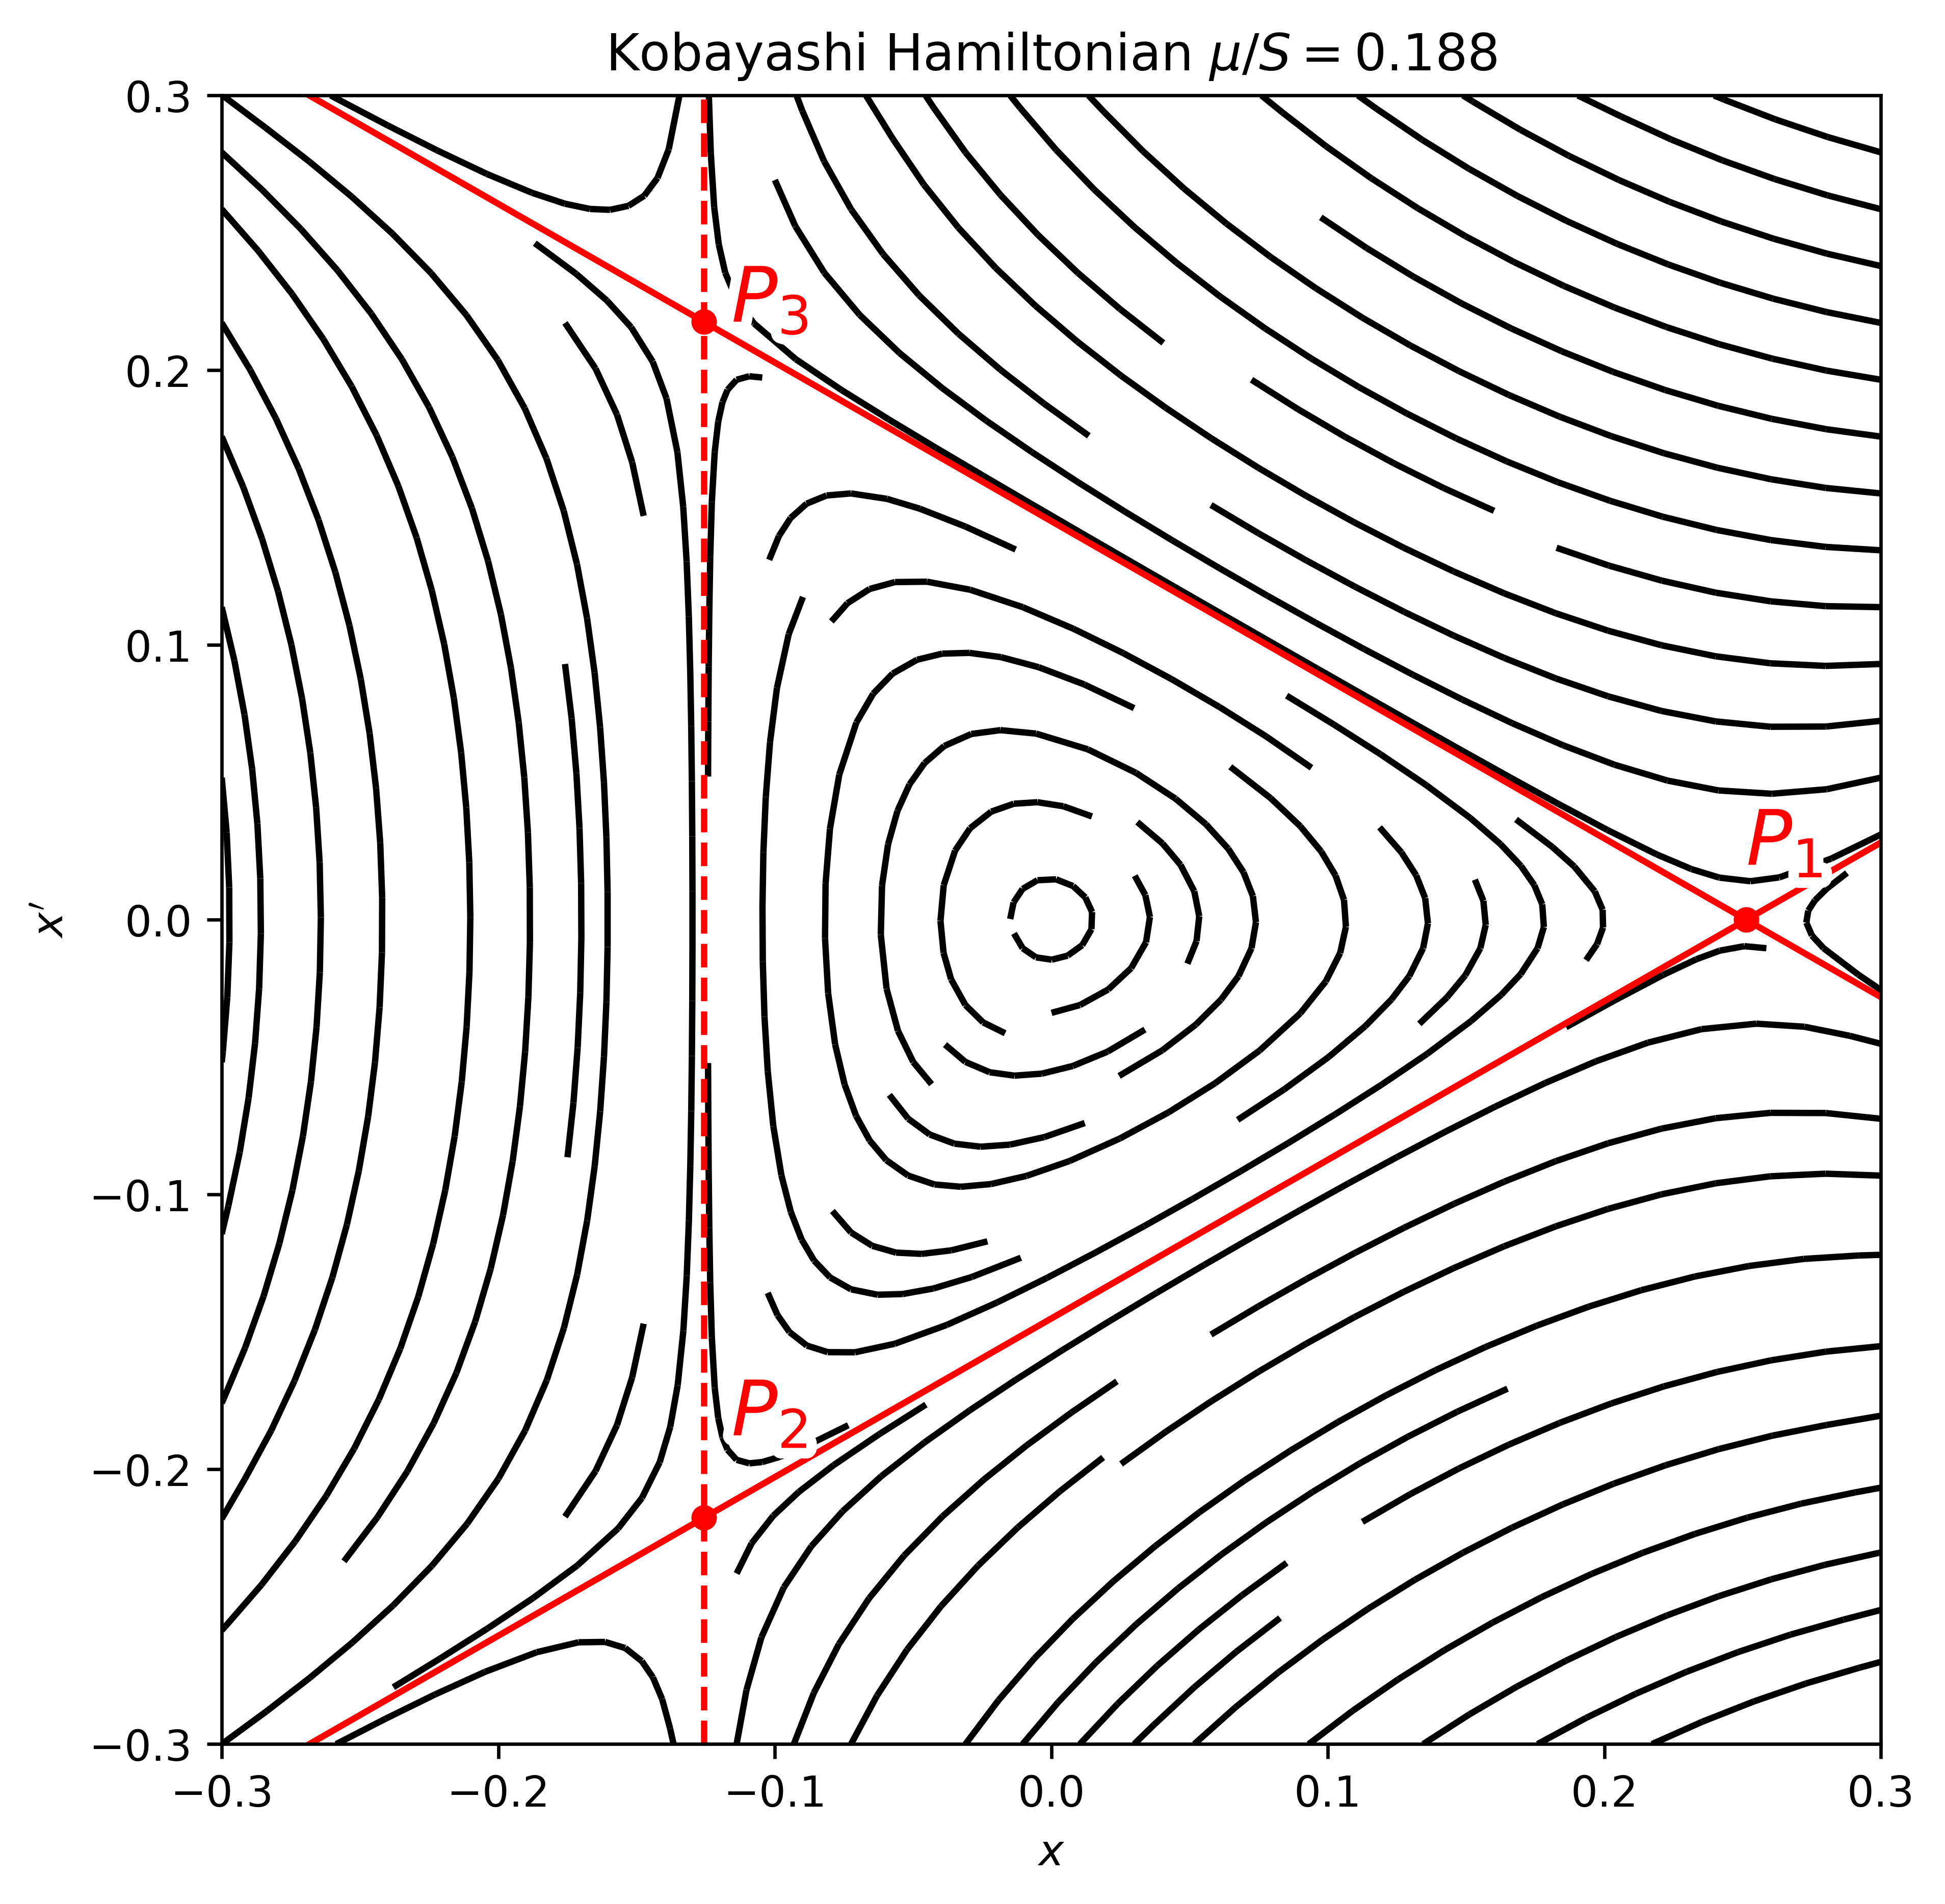
\includegraphics[width=0.6\linewidth]{kobayashi.png}
  \caption{Normalised phase-space map of the Kobayashi Hamiltonian, for a ratio $\mu/S=0.188$. The points $P_1, P_2, P_3$ are shown, with connecting lines. The value of $-h$, which defines the $P_2, P_3$ line, is dashed.}\label{fig:kobayashi}
\end{figure}

The first term describes the typical circular phase-space motion familiar from~\autoref{subsec:trans_phase_space}, with a sextupole strength $S=0$ (i.e. a linear machine). The second term describes the sextupole effect, transforming the elliptical map into a triangular trajectory for increasing values of $x$ and $x'$. The phase-space map is shown in~\autoref{fig:kobayashi}. A boundary triangle is easily identified from the map, which defines the trajectory of the stable particle with greatest possible amplitude, before the motion becomes unstable. Outside of this stable region, the particle trajectories do not close on themselves, and the particle will rapidly gain amplitude. The region bounded by this \textit{separatrix} is known as the \textit{acceptance} the size of which is defined by $|\mu /S|$, and can be found by factorising $\bf H$ at at a value of $(2\mu /3)^3/S^2$, which factorisses to three points:
\begin{eqnarray}
  P_1 &=& \left(\frac 43 \frac\mu S,    0                       \right) \\
  P_2 &=& \left(-\frac 23 \frac \mu S,  -\frac{2\mu}{\sqrt 3 S} \right) \\
  P_3 &=& \left(-\frac 23 \frac \mu S,  \frac{2\mu}{\sqrt 3 S} \right)
\end{eqnarray}
The $x$ location of the stable particle, $h$ can also be defined as
\begin{equation}
  h=\frac 23 \frac \mu S = \frac{4\pi}S\delta Q
  \label{eq:apothem}
\end{equation}
Therefore, the lines connecting $P_1, P_2$ and $P_1, P_3$, along with the vertical line at $-h$, define the separatrix. The acceptance, the area bounded by the separatrices, is defined as $A=3\sqrt 4 h^2$.

\subsection{Slow Extraction Principles}
The fundamental principle of slow extraction exploits the unstable boundary created by sextupolar fields. After a beam is injected and stable, this \textit{waiting} beam is accelerated towards the $\nicefrac 13$-integer resonance. A particle at resonance will then ``lock on'' to one of the separatrix arms, and its amplitude will grow in steps of three turns, rotating around the three separatrices. By carefully controlling the rate at which particles enter resonance, the 3-turn amplitude growth (spiral step) can be adjusted to create a desired flux of particles entering resonance. After a number of turns of amplitude growth (typically hundreds), an electrostatic septum located at some distance from the waiting beam will provide a kick necessary to extract the particles. A real-world diagram of slow extraction is shown in~\autoref{fig:real-world}.

\begin{figure}
  \centering
  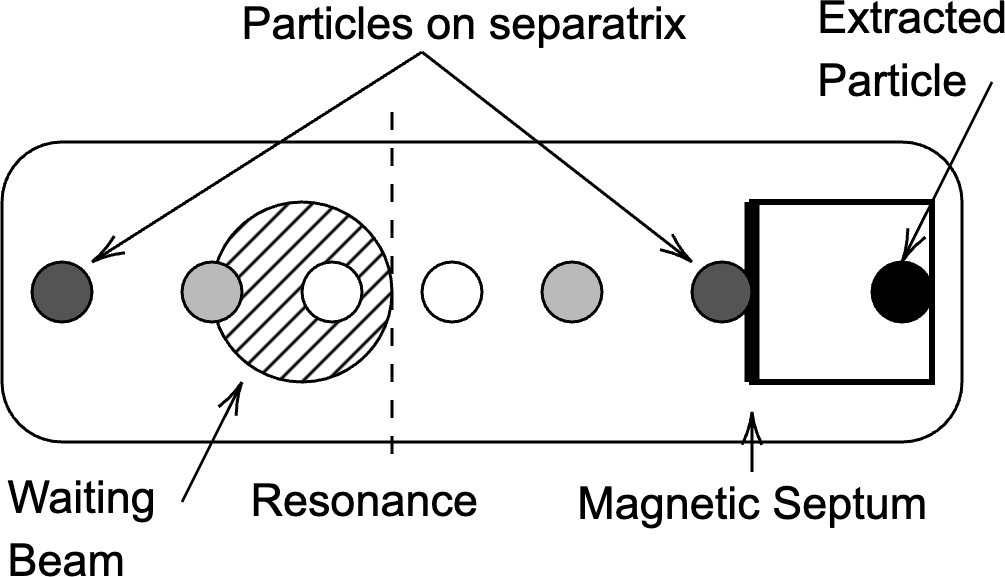
\includegraphics[width=0.6\linewidth]{real-world.png}
  \caption{A real-world diagram of momentum-driven slow extraction, looking along the $s$ direction at the magnetic septum location. The waiting beam approaches resonance (dashed), and some particles begin large turn-by-turn oscillations (increasing shaded gradient with turn number) before they jump the septum blade (thick black line) and will be extracted.}\label{fig:real-world}
\end{figure}

There are a variety of methods to provide the acceleration towards resonance, which fall into two categories: \textit{momentum-driven} methods rely on accelerating the beam towards a stationary resonance by controlling the momentum $\Delta p/p$, whereas \textit{amplitude-driven} methods use transverse noise or RF excitation at the beam's revolution frequency to create increasing betatron amplitudes.

\subsection{Steinbach Diagram}

\begin{figure}[ht]
  \centering
  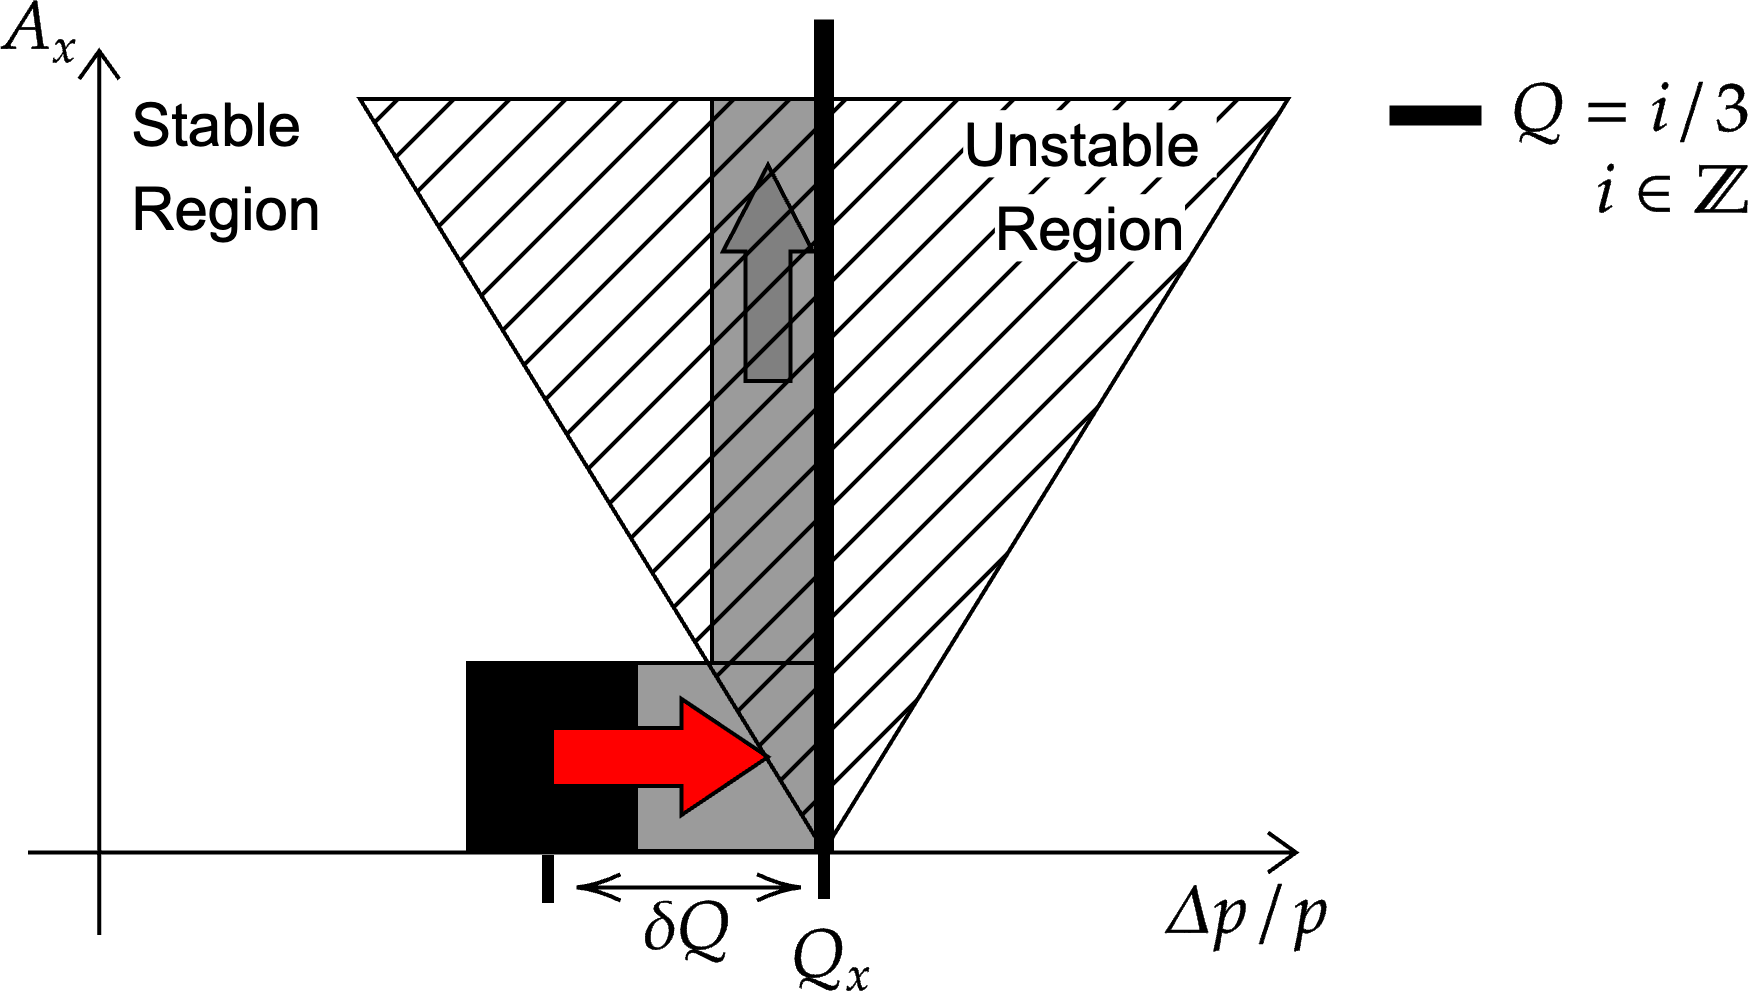
\includegraphics[width=0.6\linewidth]{momentum-driven.png}
  \caption{Stienbach diagram of momentum-driven slow extraction. Waiting beam in black, resonance driving effect in red, unstable beam in grey.}\label{fig:momentum-driven}
\end{figure}

\begin{figure}[ht]
  \centering
  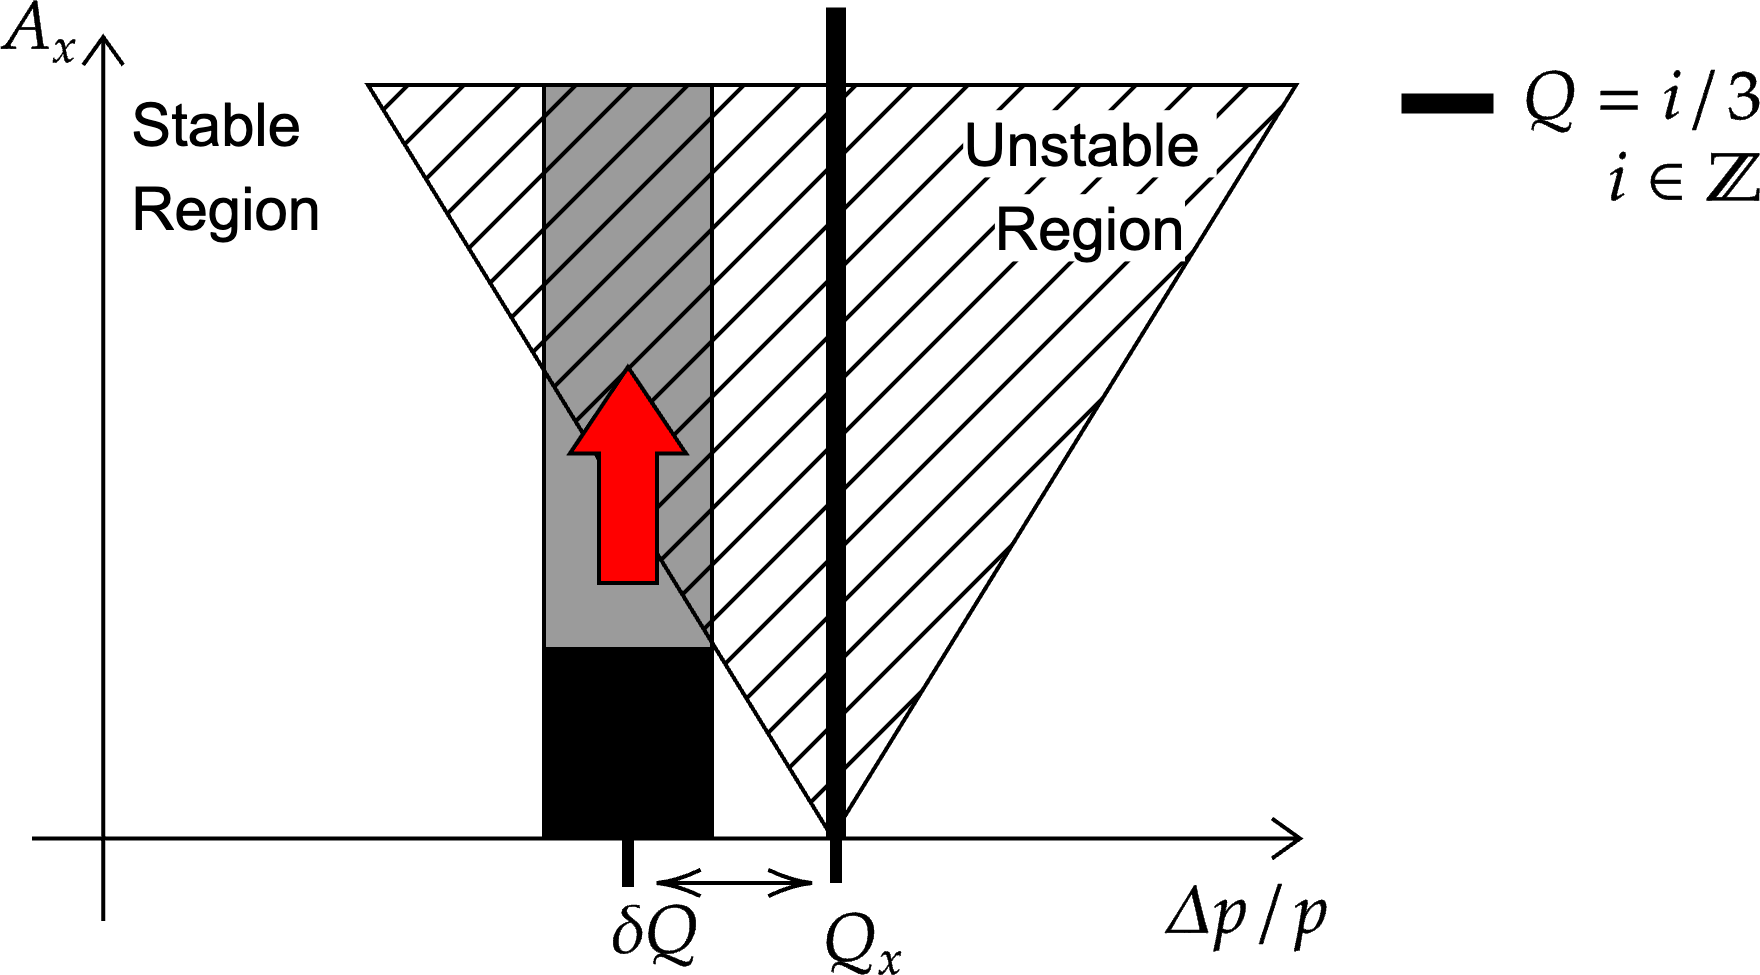
\includegraphics[width=0.6\linewidth]{amplitude-driven.png}
  \caption{Stienbach diagram of amplitude-driven slow extraction. Waiting beam in black, resonance driving effect in red, unstable beam in grey.}\label{fig:amplitude-driven}
\end{figure}

These two methods can be compared using a Stienbach\footnote{Attributed to C. Steinbach, CERN} diagram. This plots the beam amplitude $A_x$ as a function of momentum $\Delta p/p_0$. The sextupole instability is shown as a triangle, within which is the unstable region beyond the phase-space map separatrices.~\autoref{fig:momentum-driven} and~\autoref{fig:amplitude-driven} illustrate \textit{momentum} and \textit{amplitude} driven slow extraction respectively.
In order for a particle to be considered stable, its single-particle emittance $\epsilon$ must be lower or equal to the area of the separatrix triangle. Using~\autoref{eq:apothem}, this condition is expressed as
\begin{equation}
  A^2\pi\le\frac{48\sqrt 3\pi}{S^2}\delta Q^2\pi
  \label{eq:steinbach}
\end{equation} 
If this condition is plotted on a $(Q, A)$ graph, the stable triangle shown in~\autoref{fig:momentum-driven} and~\autoref{fig:amplitude-driven} is seen. The width of this unstable triangle, known as the \textit{stopband}, is proportional to $S$.

% =============================================================== %

\subsection{Slow Extraction Methods}

\subsubsection{Betatron Core}

A simple treatment of momentum-driven slow extraction is through the use of a \textit{betatron core}. Used by accelerators such as the \textit{National Center for Oncological Hadrontherapy}~\cite{Falbo:IPAC2018-TUZGBF3} (CNAO) and MedAustron~\cite{pablo}, a beatron core is a circular magnet placed around the beam to produce a longitudinal voltage along $s$. Both the CNAO and MedAustron designs, and many more medical machines, were based on a landmark report \textit{Proton-Ion Medical Machine Study}~\cite{PIMMS} (PIMMS), with the Betatron Core particularly referencing earlier work~\cite{betatroncore}.

Recalling~\autoref{eq:chroma}, a beam with non-zero (and typically negative) chromaticity $Q'$ can have its tune distance $\delta Q$ controlled by momentum $\Delta p/p$. The longitudinal voltage from the betatron core provides the resonance driving effect (red arrow in~\autoref{fig:momentum-driven}), accelerating particles into resonance. Particles then experience unstable betatron oscillation, jumping between separatrices, before encountering an electrostatic septum, where they receive an extraction kick.

\subsubsection{Tune Sweep}
Tune sweep operates somewhat as the opposite of Betatron Core: rather than controlling the beam's tune distance away from resonance ($\delta Q$), moving the beam into resonance, the reference transverse tune of the machine ($Q_x$) is moved through the stationary waiting beam. This is illustrated, with a Stienbach diagram, in~\autoref{fig:tune-sweep}.

\begin{figure}
  \centering
  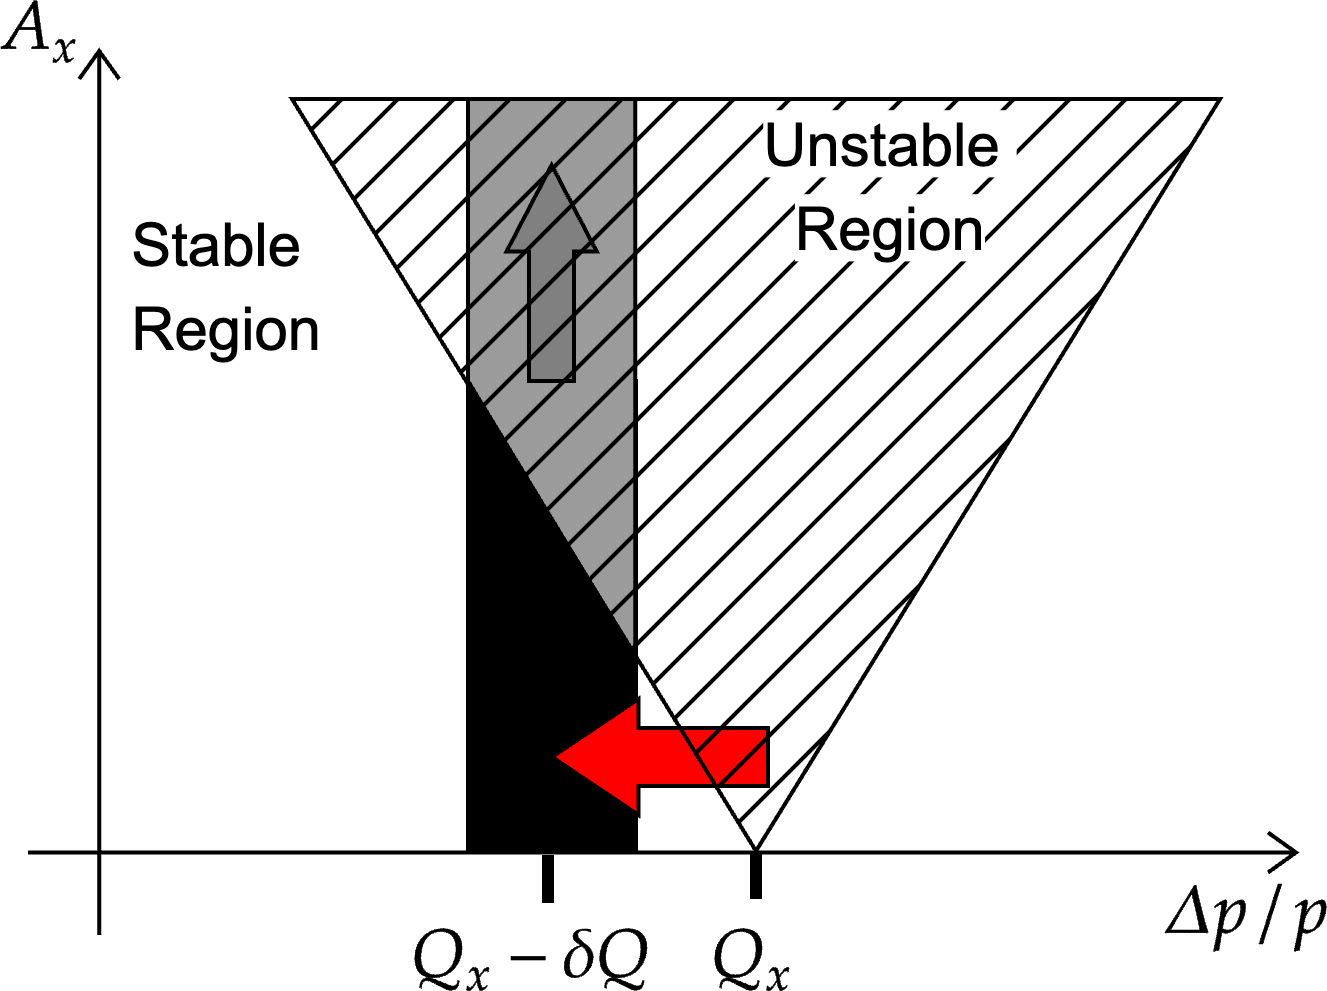
\includegraphics[width=0.6\linewidth]{tune-sweep.png}
  \caption{Stienbach diagram of tune-sweep slow extraction. Waiting beam in black, resonance driving effect in red, unstable beam in grey.}\label{fig:tune-sweep}
\end{figure}

For a small momentum spread $\Delta p/p$, the tune's dependency on quadrupole strength can be assumed as linear, so a simple quadrupole strength sweep is all that is required for tune-sweep.

There are, however disadvantages to this approach. Changing the quadrupole strength requires changing the optics of the machine, effectively creating a spread of magnetic rigidity ($B\rho$,~\autoref{eq:brho}) in the beam. The effect of this is illustrated in~\autoref{fig:hardt}: particles excited into instability with different amplitudes will ``lock on'' to separatrices at different phase-space locations. The result is a range in angle of particles extracted at the electrostatic septum (located at, for example $x=0.3$ in~\autoref{fig:hardt}).

\begin{figure}
  \centering
  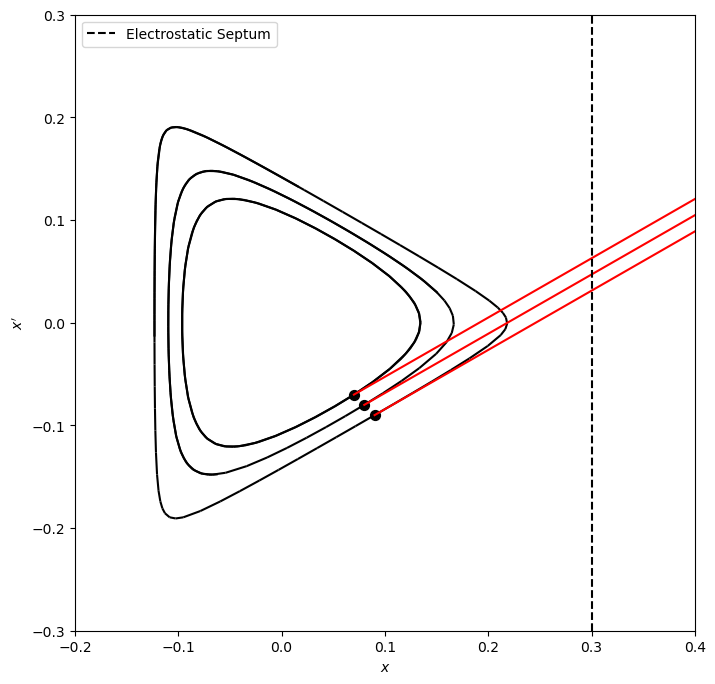
\includegraphics[width=0.6\linewidth]{hardt.png}
  \caption{Phase-space map of three initial particles on the Kobayashi Hamiltonian, and one of their separatrices. An example electrostatic septum location is shown (dashed line).}\label{fig:hardt}
\end{figure}

Recalling~\autoref{eq:steinbach}, amplitude $A$ is correlated with momentum difference $\Delta p/p$. Given a real dispersion value (\autoref{eq:dispersion}), a condition can be computed which would align all separatrices on the septum:
\begin{equation}
  D_n\cos(\pi-\Delta\phi)+D'_n\sin(\pi-\Delta\phi)=-\frac{4\pi}3Q'_x
\end{equation}
This condition, known as the Hardt condition~\cite{hardt}, will align the separatrices, given a phase advance $\Delta\phi$ and dispersion coefficients $D_n, D'_n$. However, in the context of tune-sweep extraction, the Hardt condition proves ineffective: a changing momentum will change dispersion coefficients, causing the separatrices to misalign.

\subsubsection{COSE}
To combat the effect of misaligned separatrices and differences in optics, \textit{Constant-Optics Slow Extraction} (COSE) employs techniques of both betatron core and tune-sweep: the magnetc rigidity $B\rho$ (or reference momentum) of the beam is increased simultaneously with the tune-sweep. 

This extraction method can be considered as betatron core extraction in the $p_0$ frame of reference, rather than the $p$ frame of reference. By reformulating~\autoref{eq:chroma} using $p_0$, the following equation for tune distance $\delta Q$ is obtained:
\begin{equation}
  \delta Q=Q'_x\frac{p-p_0}{p_0}
\end{equation}

\subsubsection{Radio-Frequency Knock-Out}

\subsection{Slow Extraction at the CERN PS}

\begin{enumerate}
  \item \todo{Sextupoles controlled with XSE}
  \item \todo{Quadrupoles controlled with QSE}
  \item \todo{Tune trim with PFWs}
  \item \todo{Extraction ES at 57, then 61}
  \item \todo{Down F61, into F61D}
\end{enumerate}

\begin{enumerate}
  \item \todo{Machine resonance at third order, leading to a derivation of the Kobayashi Hamiltonian and Steinbach diagram} \checkmark
  \item \todo{Betatron} \checkmark
  \item \todo{COSE (chromatic)}
  \item \todo{Q-sweep}
  \item \todo{\textbf{RFKO} INTRODUCE RFKO FORMALLY HERE}
  \item \textcolor{teal}{Mathematical description of the four regimes}
  
  \item \textcolor{teal}{Demonstrate why RFKO is of interest}
  \item \textcolor{teal}{How i actually do RFKO at the PS - the PFW, XSE, and QSE over the cycle, the beam parameters}
\end{enumerate}


\chapter{Simulation and Benchmarking}
\section{Simulation Methodology}
\todo{\textbf{Focussed on original contribution}}
\begin{enumerate}
    \item \todo{What tools are available? MAD-X, MapTrack, Henontrack, Xsuite}
    \item \todo{How do they compare?} \textcolor{teal}{Accuracy studies between basic simulations}
    \item \todo{How extraction can be implemented in them: MAD-X limitation of sub-turn frequencies; Xtrack Exciter element}
    \item \todo{How extraction compares} \textcolor{teal}{spill accuracy studies between simulations and machine data}
    \item \todo{How performance compares} \textcolor{teal}{performance studies between SX simulations on CPU and GPGPU}
\end{enumerate}

\chapter{Conclusion}


TEST
\chapter{Acknowledgements}

\bibliographystyle{IEEEtran} 
\bibliography{refs} 

\begin{appendices}

\chapter{Derivations}

\section{Relating longitudinal variables}

In order to relate the dispersive and chromatic functions produced by \verb|MAD-X| to those calculated by \verb|Xtrack|, we must multiply \verb|MAD-X|'s results by the relativistic Lorentz factor $\beta=v/c$. This is because \verb|MAD-X| uses the relative momentum error $\delta_p$ as a longitudinal variable, defined as
\begin{equation}
\delta_p=\frac{p-p_0}{p_0}
\end{equation}, where $p$ is the momentum of the particle, and $p_0$ the momentum of the {\it reference} (or {\it design}) particle, whereas \verb|Xtrack| uses the relative energy error

\chapter{Code Snippets}

\chapter{Data and Plots}

\end{appendices}

\end{document}
